\documentclass[slidestop,compress,xcolor=table,mathserif,hyperref={bookmarks=false}]{beamer}
\usetheme{TACC}

\usepackage{tikz}
\usetikzlibrary{automata,shapes,arrows}
\usepackage{lmodern}
\usepackage[overlay]{textpos}
\usepackage[applemac]{inputenc}
\usepackage{pgfpages}
\usepackage{multirow}

\newenvironment<>{varblock}[2][.9\textwidth]{
  \setlength{\textwidth}{#1}
  \begin{actionenv}#3
    \def\insertblocktitle{#2}
    \par
    \usebeamertemplate{block begin}}
  {\par
    \usebeamertemplate{block end}
  \end{actionenv}}

\author{\textbf{\Large Jim Browne, Ashay Rane and Leo Fialho}}
\begin{document}

\AtBeginSection[]{
	\frame<beamer>{
		\frametitle{Agenda}
		\begin{columns}[c]
			\begin{column}{0.6\textwidth}
				\tableofcontents[currentsection,subsectionstyle=shadow/hide/hide]
			\end{column}
			\begin{column}{0.5\textwidth}
				\pgfuseimage{configuration}
			\end{column}
		\end{columns}
	}
}

%------------------------------------------------------------
\pgfdeclareimage[interpolate=true,width=5cm]{logo_TACC}{figures/tacc}
\pgfdeclareimage[interpolate=true,width=5cm]{logo_UT}{figures/ut}
\pgfdeclareimage[interpolate=true,width=1.5cm]{logo_TACC_small}{figures/tacc}
\pgfdeclareimage[interpolate=true,width=1cm]{logo_UT_small}{figures/ut}
\pgfdeclareimage[interpolate=true,width=6cm]{configuration}{figures/configuration}

%------------------------------------------------------------
\title{\textbf{\Huge PerfExpert}}
\date{\textbf{\huge TACC Summer Supercomputing Institute} \\ \ \\ \ \\ \pgfuseimage{logo_TACC} \ \ \pgfuseimage{logo_UT}}
\logo{\pgfuseimage{logo_TACC_small} \ \ \ \pgfuseimage{logo_UT_small}}
\frame[plain]{\titlepage}

%------------------------------------------------------------
\section{Introduction}

\subsection{Overview}
\frame{\frametitle{Overview: why PerfExpert?} %\pause
	\begin{block}{Problem: HPC systems operate far below peak} %\pause
		\begin{itemize}
			\item Chip/node architectural complexity is growing rapidly \\[2mm] %\pause
			\item Performance optimization for these chips requires deep knowledge of architectures, code patterns, compilers, etc. \\[2mm]
		\end{itemize}
	\end{block}

	\begin{exampleblock}{Performance optimization tools} %\pause
		\begin{itemize}
			\item Powerful in the hands of experts \\[2mm] %\pause
			\item Require detailed performance and system expertise \\[2mm] %\pause
			\item HPC application developers are domain experts, not computer gurus \\[2mm] %\pause
		\end{itemize}
	\end{exampleblock}

	\begin{alertblock}{Result: Many HPC programmers do not use these tools}
		\centering (seriously)
	\end{alertblock}
}

\frame{\frametitle{Goal for PerfExpert: democratize optimization!} %\pause
	\begin{block}{Subgoals:} %\pause
		\begin{itemize}
			\item Make use of the tool as simple as possible \\[2mm] %\pause
			\item Start with only chip/node level optimization \\[2mm] %\pause
			\item Make it adaptable across multiple architectures \\[2mm] %\pause
			\item Design for extension to communication and I/O performance \\[2mm] %\pause
		\end{itemize}
	\end{block}

	\begin{exampleblock}{How to accomplish?} %\pause
		\begin{itemize}
			\item Formulate the performance optimization task as a workflow of subtasks \\[2mm] %\pause
			\item Leverage the state-of-the-art: build on the best available tools for the subtasks to minimize the effort and cost of development \\[2mm] %\pause
			\item Automate the entire workflow \\[2mm] %\pause
		\end{itemize}
	\end{exampleblock}
}

\subsection{Introduction}
\frame{\frametitle{Introduction}
	\begin{block}{The four stages of automatic performance optimization:} %\pause
		\begin{itemize}
			\item Measurement and attribution (1) \\[2mm] %\pause
			\item Analysis, diagnosis and identification of bottlenecks (2) \\[2mm] %\pause
			\item Selection of effective optimizations (3) \\[2mm] %\pause
			\item Implementation of optimizations (4) \\[2mm] %\pause
		\end{itemize}
	\end{block}

	\begin{exampleblock}{Use of State-of-the-Art:} %\pause
		\begin{itemize}
			\item HPCToolkit/Intel VTune, \textbf{MACPO} based on ROSE (1) \\[2mm] %\pause
			\item \textbf{PerfExpert Team} (2 and 3) \\[2mm] %\pause
			\item \textbf{PerfExpert Team} based on ROSE, PIPS, Bison and Flex (4)\\[2mm] %\pause
		\end{itemize}
	\end{exampleblock}
}

\frame{\frametitle{Introduction}
	\begin{block}{Uniqueness of PerfExpert:} %\pause
		\begin{itemize}
			\item Nearly complete optimization first three stages of optimization for chip/node level \\[2mm] %\pause
			\item Framework for implementing optimizations is complete and several optimizations are completed \\[2mm] %\pause
			\item Integrates code segment focused and data structure based measurements (\textbf{MACPO})\\[2mm] %\pause
			\item Workflow will apply to communication and I/O optimization as well \\[2mm] %\pause
		\end{itemize}
	\end{block}
}

\frame{\frametitle{Introduction}
	\begin{block}{Unique properties of MACPO (integrated into PerfExpert):} %\pause
		\begin{itemize}
			\item Multicore resolved traces \\[2mm] %\pause
			\item Code segment local measurement \\[2mm] %\pause
			\item Data structure specific traces \\[2mm] %\pause
			\item Order of magnitude lower overhead of measurement \\[2mm] %\pause
			\item More accurate (associative) cache models \\[2mm] %\pause
			\item Strides by data structure and code segment \\[2mm] %\pause
			\item Architecture ``independent'' metrics \\[2mm]
		\end{itemize}
	\end{block}
}

\subsection{What PerfExpert can provide to you?}

\frame{\frametitle{What PerfExpert can provide to you?}
	\begin{block}{Performance report:} %\pause
		\begin{itemize}
			\item Identification of bottlenecks by relevance \\[2mm] %\pause
			\item Performance analysis based on performance metrics \\[2mm] %\pause
			\item Recommendations for optimization \\[2mm] %\pause
		\end{itemize}
	\end{block}

	\begin{exampleblock}{There are three possible outputs:} %\pause
		\begin{itemize}
			\item Performance report only \\[2mm] %\pause
			\item List of recommendations \\[2mm] %\pause
			\item Fully automated code transformation \\[2mm]
		\end{itemize}
	\end{exampleblock}
}

\frame{\frametitle{Performance Report}
	\begin{block}{}
\texttt{\tiny Loop in function compute() at mm.c:8 (99.8\% of the total runtime)\\
===============================================================================\\
ratio to total instrns \ \ \ \ \ \ \%  0.........25...........50.........75........100\\
\ \ \ - floating point \ \ \ \ \ : \ 100 ***********************************************\\
\ \ \ - data accesses \ \ \ \ \ \ : \ \ 25 ************\\
* GFLOPS (\% max) \ \ \ \ \ \ \ \ : \ \ 12 ******\\
\ \ \ - packed \ \ \ \ \ \ \ \ \ \ \ \ \ : \ \ \ 0 *\\
\ \ \ - scalar \ \ \ \ \ \ \ \ \ \ \ \ \ : \ \ 12 ******\\
-------------------------------------------------------------------------------\\
performance assessment \ \ \ \ LCPI good......okay......fair......poor......bad....\\
* overall \ \ \ \ \ \ \ \ \ \ \ \ \ \ \ : \ 3.0 >>>>>>>>>>>>>>>>>>>>>>>>>>>>>>>>>>>>>>>>>>>>>>+\\
upper bound estimates\\
* data accesses \ \ \ \ \ \ \ \ \ : \ 9.6 >>>>>>>>>>>>>>>>>>>>>>>>>>>>>>>>>>>>>>>>>>>>>>+\\
\ \ \ - L1d hits \ \ \ \ \ \ \ \ \ \ \ : \ 0.9 >>>>>>>>>>>>>>>>>\\
\ \ \ - L2d hits \ \ \ \ \ \ \ \ \ \ \ : \ 1.8 >>>>>>>>>>>>>>>>>>>>>>>>>>>>>>>>>>>>>\\
\ \ \ - L2d misses \ \ \ \ \ \ \ \ \ : \ 6.9 >>>>>>>>>>>>>>>>>>>>>>>>>>>>>>>>>>>>>>>>>>>>>>+\\
* instruction accesses \ \ : \ 0.1 >\\
\ \ \ - L1i hits \ \ \ \ \ \ \ \ \ \ \ : \ 0.0 >\\
\ \ \ - L2i hits \ \ \ \ \ \ \ \ \ \ \ : \ 0.0 >\\
\ \ \ - L2i misses \ \ \ \ \ \ \ \ \ : \ 0.1 >\\
* data TLB \ \ \ \ \ \ \ \ \ \ \ \ \ \ : \ \ 4.6 >>>>>>>>>>>>>>>>>>>>>>>>>>>>>>>>>>>>>>>>>>>>>>+\\
* instruction TLB \ \ \ \ \ \ \ : \ \ 0.0 >\\
* branch instructions \ \ \ : \ 0.1 >>\\
\ \ \ - correctly predicted : \ 0.1 >>\\
\ \ \ - mispredicted \ \ \ \ \ \ \ : \ 0.0 >\\
* floating-point instr \ \ : \ 5.1 >>>>>>>>>>>>>>>>>>>>>>>>>>>>>>>>>>>>>>>>>>>>>>+\\
\ \ \ - fast FP instr \ \ \ \ \ \ : \ 5.1 >>>>>>>>>>>>>>>>>>>>>>>>>>>>>>>>>>>>>>>>>>>>>>+\\
\ \ \ - slow FP instr \ \ \ \ \ \ : \ 0.0 >\\
}
   \end{block}
}

\frame{\frametitle{List of Recommendations}
	\begin{block}{}
\texttt{\small \#--------------------------------------------------\\
\# Recommendations for mm.c:8\\
\#--------------------------------------------------\\
\# This is a possible recommendation for this code segment\\
\#\\
Description: change the order of loops\\
Reason: this optimization may improve the memory access pattern and make it more cache and TLB friendly\\
Pattern Recognizers: c\_loop2 f\_loop2 \\
Code example:\\
loop i \{\\
\ \ loop j \{...\}\\
\}\\
 =====>
loop j \{\\
\ \ loop i \{...\}\\
\}\\
}
	\end{block}
}

\frame{\frametitle{Fully Automated Code Transformation}
	\begin{columns}[c]
		\begin{column}{0.5\textwidth}
			\begin{block}{Before:}
\texttt{\scriptsize void compute() \{\\
\ register int i, j, k;\\
\ \\
\ \\
\ \\
\ \\
\ \\
\ for (i = 0; i < 1000; i++)\\
\ \\
\ \\
\ \ for (j = 0; j < 1000; j++)\\
\ \\
\ \ \ for (k = 0; k < 1000; k++)\\
\ \ \ \ c[i][j] += (a[i][k] * b[k][j]);\\
\}\\
}
			\end{block}
		\end{column}
		\begin{column}{0.5\textwidth}
			\begin{block}{After:}
\texttt{\scriptsize void compute() \{\\
\ register int i, j, k;\\
\textcolor{red}{\ //PIPS generated variable}\\
\textcolor{red}{\ register int jp, kp;}\\
\textcolor{red}{\ /* PERFEXPERT: start work here */}\\
\textcolor{red}{\ /* PERFEXPERT: grandparent loop */}\\
\textcolor{red}{\ loop\_6:}\\
\textcolor{blue}{\ for (i = 0; i <= 999; i++)}\\
\textcolor{red}{\ \ /* PERFEXPERT: parent loop */}\\
\textcolor{red}{\ \ loop\_7:}\\
\textcolor{blue}{\ \ for(jp = 0; jp <= 999; jp += 1)}\\
\textcolor{red}{\ \ \ /* PERFEXPERT: bottleneck */}\\
\textcolor{blue}{\ \ \ for(kp = 0; kp <= 999; kp += 1)}\\
\textcolor{blue}{\ \ \ c[i][kp] += a[i][jp]*b[jp][kp];}\\
\}\\
}
			\end{block}
		\end{column}
	\end{columns}
}

%------------------------------------------------------------
\section{The User Perspective}
\subsection{The User Perspective}

\frame{\frametitle{Basic Usage of PerfExpert}
	\begin{block}{Making PerfExpert Available} %\pause
		\texttt{\$ module load papi perfexpert} \\[2mm] %\pause
	\end{block}
	\begin{block}{Execution Options} %\pause
		\texttt{\small Usage: perfexpert [-ghmvq] [-w DIR] [-s FILE] [-r COUNT]\\
\ \ \ \ \ \ \ \ \ \ \ \ \ \ \ \ \ \ \ program\_executable [program\_arguments]\\
\ \\
-s \ \ \ Use FILE as the source code\\
-m \ \ \ Use `make' to compile source code\\
-q \ \ \ Disable verbose mode\\
-w \ \ \ Use DIR as temporary directory\\
-g \ \ \ Do not remove the temporary directory\\
-r \ \ \ Use COUNT as the number of recommendation to show\\
\ \\
  Use CC, CFLAGS and LDFLAGS to select compiler and compilation/linkage flags} \\[2mm] %\pause
	\end{block}
}

\frame{\frametitle{Basic Usage of PerfExpert}
	\tikzstyle{decision} = [diamond, draw, fill=blue!20, text width=0.8cm, text badly centered]
	\tikzstyle{block} = [rectangle, draw, fill=blue!20, text width=2cm, text centered, rounded corners]
	\tikzstyle{line} = [draw, -stealth']
	\tikzstyle{cloud} = [draw, ellipse,fill=red!20]

	\begin{tikzpicture}[node distance=1cm,auto]\small
		\node [cloud] (perfexpert) {perfexpert};
		\node [decision, right of=perfexpert, node distance=3cm] (dashS) {\small If -s};
		\node [decision, right of=dashS, node distance=2.5cm] (dashM) {\small If -m};
		\node [block, right of=dashM, node distance=3cm] (make) {Run\\ \texttt{\small make}};
		\node [block, below of=make, node distance=1.5cm] (cc) {\texttt{\small CC source.c}};
		\node [block, left of=cc, node distance=3cm] (binary) {\small Binary Object};
		\node [block, left of=binary, node distance=2.5cm] (run) {\small Run Experiment};
		\node [decision, below of=run, node distance=1.75cm] (dashS2) {\small If -s};
		\node [decision, below of=dashS2, node distance=2cm] (dashR) {\small If -r};
		\node [block, left of=dashR, node distance=2.5cm] (analysis) {\small Show Analysis};
		\node [block, right of=dashS2, node distance=2.5cm] (auto) {\small Auto Optimization};
		\node [block, right of=auto, node distance=3cm] (analysis2) {\small Show Analysis};
		\node [block, right of=dashR, node distance=2.5cm] (recom) {\small Show Recommend.};
		\node [cloud, below of=dashR, node distance=1.5cm] (end) {end};
		\path [line] (perfexpert) -- (dashS);
		\path [line] (dashS) -- node {yes} (dashM);
		\path [line] (dashM) -- node {yes} (make);
		\path [line] (dashS) -- node {no} (binary);
		\path [line] (make) -- (cc);
		\path [line] (dashM) -- node {no} (cc);
		\path [line] (cc) -- (binary);
		\path [line] (binary) -- (run);
		\path [line] (run) -- (dashS2);
		\path [line] (dashS2) -- node {yes} (auto);
		\path [line] (dashS2) -- node {no} (dashR);
		\path [line] (auto) -- (binary);
		\path [line] (dashR) -- node {yes} (recom);
		\path [line] (dashR) -- node {no} (analysis);
		\path [line,dashed] (auto) -- (analysis2);
		\path [line,dashed] (analysis2) |- (recom);
		\path [line] (analysis) |- (end);
		\path [line] (recom) |- (end);	
	\end{tikzpicture}
}

\frame{\frametitle{Basic Usage of PerfExpert}
	\begin{block}{In Other Words...} %\pause
		\begin{itemize}
			\item No source code, no automatic optimization \\[1mm] %\pause
			\item No source code, choose between analysis or recommendation \\[1mm] %\pause
			\item Source code, enable automatic optimization \\[1mm] %\pause
			\item Source code, choose the compilation method (-m) and options (CC, CFLAGS and LDFLAGS)\\[1mm] %\pause
			\item Source code, show analysis and recommendation after all the possible automatic optimizations have been applied \\
		\end{itemize}
	\end{block}
	\begin{exampleblock}{Examples:} %\pause
		\texttt{\small \$ perfexpert my\_program param1 param2} \\ %\pause
		\texttt{\small \$ perfexpert -r 5 my\_program param1 param2} \\ %\pause
		\texttt{\small \$ perfexpert -s my\_program.c my\_program param1 param2} \\ %\pause
		\texttt{\small \$ perfexpert -m -s my\_program.c my\_program param1 param2} \\  %\pause
	\end{exampleblock}
}

\frame{\frametitle{Understanding PerfExpert Analysis}
	\begin{block}{On the The Analysis Report...} %\pause
		\begin{itemize}
			\item The more ``expensive'' comes first \\[2mm] %\pause
			\item Tells user where the slow code sections are as well as why they perform poorly \\[2mm] %\pause
			\item Every function or loop which takes more than 1\% of the execution time is analyzed (default value) \\[2mm] %\pause
			\item Yes, we rely on performance metrics (but not only and not the raw ones) \\[2mm] %\pause
			\item No, we do not rely on hardware specs \\[2mm] %\pause
			\item If you are not using properly the node PerfExpert may conclude everything is fine (use a representative workload) \\[2mm] %\pause
		\end{itemize}
	\end{block}
}

\frame{\frametitle{Metrics used by PerfExpert} %\pause
	\begin{block}{Source Code} %\pause
		\begin{itemize}
			\item Language (C, C++, Fortran) \\[2mm] %\pause
			\item File name and line number \\[2mm] %\pause
			\item Type (loop or function) \\[2mm] %\pause
			\item Function name and ``deepness'' \\[2mm] %\pause
			\item Representativeness (percentage of execution time) \\[2mm]
		\end{itemize}
	\end{block}
	\begin{block}{Execution Performance} %\pause
		\begin{itemize}
			\item Raw data (PAPI) \\[2mm] %\pause
			\item LCPI: local cycles per instruction (PerfExpert Analyzer) \\[2mm]
		\end{itemize}
	\end{block}
}
\frame{\frametitle{Metrics used by PerfExpert} %\pause
	\begin{block}{Architecture Characteristics} %\pause
		\begin{itemize}
			\item Memory access latency: L1, L2, L3 and main memory (based on micro-benchmarks) \\[2mm] %\pause
			\item Memory hierarchy, topology and size (based on hwlock) \\[2mm] %\pause
			\item Branch latency and missed branch latency (based on micro-benchmarks) \\[2mm] %\pause
			\item Float-point operation latency (based on micro-benchmarks) \\[2mm] %\pause
			\item Micro-architecture \textcolor{red}{(in progress)} \\[2mm]
		\end{itemize}
	\end{block}
}
\frame{\frametitle{Metrics used by PerfExpert} %\pause
	\begin{block}{Data Access Performance (from MACPO)} %\pause
		\begin{itemize}
			\item Access strides and the frequency of occurrence (*) \\[2mm] %\pause
			\item Presence or absence of cache thrashing and the frequency (*) \\[2mm] %\pause
			\item Estimated cost (cycles) per access (*) \\[2mm] %\pause
			\item NUMA misses (*) \\[2mm] %\pause
			\item Reuse factors for data caches (*) \\[2mm] %\pause
			\item Stream count \\[2mm]
		\end{itemize}
	\end{block}
	(*) \textit{per variable}
}

\frame{\frametitle{Performance Report}
	\begin{block}{}
\texttt{\tiny Loop in function compute() at mm.c:8 (99.8\% of the total runtime)\\
===============================================================================\\
ratio to total instrns \ \ \ \ \ \ \%  0.........25...........50.........75........100\\
\ \ \ - floating point \ \ \ \ \ : \ 100 ***********************************************\\
\ \ \ - data accesses \ \ \ \ \ \ : \ \ 25 ************\\
}
	\end{block}
	\begin{block}{Interpretation}
		\begin{itemize}
			\item What percentage of the total instructions were computational (floating-point instructions) \\[2mm] %\pause
			\item What percentage were instructions that accessed data \\[2mm] %\pause
			\item So, whether optimizing the program for either data accesses or floating-point instructions would have a significant impact on the total running time of the program? \\[2mm]
		\end{itemize}
	\end{block}
}

\frame{\frametitle{Performance Report}
	\begin{block}{}
\texttt{\tiny Loop in function compute() at mm.c:8 (99.8\% of the total runtime)\\
...\\
* GFLOPS (\% max) \ \ \ \ \ \ \ \ : \ \ 12 ******\\
\ \ \ - packed \ \ \ \ \ \ \ \ \ \ \ \ \ : \ \ \ 0 *\\
\ \ \ - scalar \ \ \ \ \ \ \ \ \ \ \ \ \ : \ \ 12 ******\\
...\\
}
	\end{block}
	\begin{block}{Interpretation}
		\begin{itemize}
			\item GFLOPs rating, which is the number of floating-point operations executed per second \\[2mm] %\pause
			\item This metric is displayed as a percentage of the maximum possible GFLOP value for that particular machine \\[2mm] %\pause
			\item It is rare for real-world programs to match even 50\% of the maximum value \\[2mm]
		\end{itemize}
	\end{block}
}

\frame{\frametitle{Performance Report}
	\begin{block}{}
\texttt{\tiny Loop in function compute() at mm.c:8 (99.8\% of the total runtime)\\
...\\
performance assessment \ \ \ \ LCPI good......okay......fair......poor......bad....\\
* overall \ \ \ \ \ \ \ \ \ \ \ \ \ \ \ : \ 3.0 >>>>>>>>>>>>>>>>>>>>>>>>>>>>>>>>>>>>>>>>>>>>>>+\\
...\\
}
   \end{block}
	\begin{block}{Interpretation}
		\begin{itemize}
			\item LCPI values: is the ratio of cycles spent in the code segment for a specific category, divided by the total number of instructions in the code segment \\[2mm] %\pause
			\item The overall value is the ratio of the total cycles taken by the code segment to the total instructions executed in the code segment \\[2mm] %\pause
			\item Generally, a value of 0.5 or lower for the CPI is considered to be good \\[2mm]
		\end{itemize}
	\end{block}
}

\frame{\frametitle{Performance Report}
	\begin{block}{}
\texttt{\tiny Loop in function compute() at mm.c:8 (99.8\% of the total runtime)\\
...\\
* data accesses \ \ \ \ \ \ \ \ \ : \ 9.6 >>>>>>>>>>>>>>>>>>>>>>>>>>>>>>>>>>>>>>>>>>>>>>+\\
\ \ \ - L1d hits \ \ \ \ \ \ \ \ \ \ \ : \ 0.9 >>>>>>>>>>>>>>>>>\\
\ \ \ - L2d hits \ \ \ \ \ \ \ \ \ \ \ : \ 1.8 >>>>>>>>>>>>>>>>>>>>>>>>>>>>>>>>>>>>>\\
\ \ \ - L2d misses \ \ \ \ \ \ \ \ \ : \ 6.9 >>>>>>>>>>>>>>>>>>>>>>>>>>>>>>>>>>>>>>>>>>>>>>+\\
* instruction accesses \ \ : \ 0.1 >\\
\ \ \ - L1i hits \ \ \ \ \ \ \ \ \ \ \ : \ 0.0 >\\
\ \ \ - L2i hits \ \ \ \ \ \ \ \ \ \ \ : \ 0.0 >\\
\ \ \ - L2i misses \ \ \ \ \ \ \ \ \ : \ 0.1 >\\
...\\
}
   \end{block}
	\begin{block}{Interpretation}
		\begin{itemize}
			\item LCPI arising from accesses to memory for program variables \\[2mm] %\pause
			\item LCPI arising from memory accesses for code (functions and loops) \\[2mm] %\pause
			\item Shows different levels of memory (L1, L2, etc.) \\[2mm]
		\end{itemize}
	\end{block}
}

\frame{\frametitle{Performance Report}
	\begin{block}{}
\texttt{\tiny Loop in function compute() at mm.c:8 (99.8\% of the total runtime)\\
...\\
* data TLB \ \ \ \ \ \ \ \ \ \ \ \ \ \ : \ \ 4.6 >>>>>>>>>>>>>>>>>>>>>>>>>>>>>>>>>>>>>>>>>>>>>>+\\
* instruction TLB \ \ \ \ \ \ \ : \ \ 0.0 >\\
* branch instructions \ \ \ : \ 0.1 >>\\
\ \ \ - correctly predicted : \ 0.1 >>\\
\ \ \ - mispredicted \ \ \ \ \ \ \ : \ 0.0 >\\
* floating-point instr \ \ : \ 5.1 >>>>>>>>>>>>>>>>>>>>>>>>>>>>>>>>>>>>>>>>>>>>>>+\\
\ \ \ - fast FP instr \ \ \ \ \ \ : \ 5.1 >>>>>>>>>>>>>>>>>>>>>>>>>>>>>>>>>>>>>>>>>>>>>>+\\
\ \ \ - slow FP instr \ \ \ \ \ \ : \ 0.0 >\\
}
   \end{block}
	\begin{block}{Interpretation}
		\begin{itemize}\small
			\item Data TLB: provides an approximate measure of penalty arising from strides in accesses or regularity of accesses \\[0mm] %\pause
			\item Instruction TLB: reflects penalty from fetching instructions due to irregular accesses \\[0mm] %\pause
			\item Branch instructions: counts penalty from jumps (i.e. if statements, loop conditions, etc.) \\[0mm] %\pause
			\item Floating-point instructions: counts LCPI from executing computational (floating-point) instructions \\[0mm] %\pause
%			\item For floating-point instructions, the division is based on floating-point instructions that take few cycles to execute (e.g. add, subtract and multiply instructions) and on floating-point instructions that take longer to execute (e.g. divide and square-root instructions) \\[0mm]
		\end{itemize}
	\end{block}
}

\frame{\frametitle{A Simple Example}
	\begin{block}{Automatic Optimization of a C Code}
		\texttt{\$ perfexpert -s code.c code}
	\end{block}
	\begin{exampleblock}{Optimization Steps}
		\begin{itemize}\small
			\item One full optimization cycle \\[2mm] %\pause
			\item Runs out of automatic optimizations during the second cycle \\[2mm] %\pause
			\item Shows the analysis report as well as recommendations \\[2mm] %\pause
			\item Execution time: from 88.856 seconds to 6.967 seconds \\[2mm] %\pause
			\item There is (still) room for improvement \\[2mm] %\pause
		\end{itemize}
	\end{exampleblock}
}

\frame{\frametitle{Comparing Codes}
	\begin{columns}[c]
		\begin{column}{0.5\textwidth}
			\begin{block}{Before:}
\texttt{\scriptsize void compute() \{\\
\ register int i, j, k;\\
\ \\
\ \\
\ \\
\ \\
\ \\
\ for (i = 0; i < 1000; i++)\\
\ \\
\ \\
\ \ for (j = 0; j < 1000; j++)\\
\ \\
\ \ \ for (k = 0; k < 1000; k++)\\
\ \ \ \ c[i][j] += (a[i][k] * b[k][j]);\\
\}\\
}
			\end{block}
		\end{column}
		\begin{column}{0.5\textwidth}
			\begin{block}{After:}
\texttt{\scriptsize void compute() \{\\
\ register int i, j, k;\\
\textcolor{red}{\ //PIPS generated variable}\\
\textcolor{red}{\ register int jp, kp;}\\
\textcolor{red}{\ /* PERFEXPERT: start work here */}\\
\textcolor{red}{\ /* PERFEXPERT: grandparent loop */}\\
\textcolor{red}{\ loop\_6:}\\
\textcolor{blue}{\ for (i = 0; i <= 999; i++)}\\
\textcolor{red}{\ \ /* PERFEXPERT: parent loop */}\\
\textcolor{red}{\ \ loop\_7:}\\
\textcolor{blue}{\ \ for(jp = 0; jp <= 999; jp += 1)}\\
\textcolor{red}{\ \ \ /* PERFEXPERT: bottleneck */}\\
\textcolor{blue}{\ \ \ for(kp = 0; kp <= 999; kp += 1)}\\
\textcolor{blue}{\ \ \ c[i][kp] += a[i][jp]*b[jp][kp];}\\
\}\\
}
			\end{block}
		\end{column}
	\end{columns}
}

\frame{\frametitle{Comparing Reports}
	\begin{columns}[c]
		\begin{column}{0.5\textwidth}\vspace{-0.5cm}
			\begin{block}{Before: 88.856 sec}
\texttt{\scriptsize ratio to total instrns \ \ \ \ \ \ \ \% \\
\ \ \ - floating point \ \ \ \ \ : \ 100 \\
\ \ \ - data accesses \ \ \ \ \ \ : \ \ 25 \\
* GFLOPS (\% max) \ \ \ \ \ \ \ \ : \ \ 13 \\
\ \ \ - packed \ \ \ \ \ \ \ \ \ \ \ \ \ : \ \ \ 0 \\
\ \ \ - scalar \ \ \ \ \ \ \ \ \ \ \ \ \ : \ \ 13 \\
--------------------------------- \\
performance assessment \ \ \ \ \ LCPI \\
* overall \ \ \ \ \ \ \ \ \ \ \ \ \ \ \ : \ 3.7 \\
* data accesses \ \ \ \ \ \ \ \ \ : 40.6 \\
\ \ \ - L1d hits \ \ \ \ \ \ \ \ \ \ \ : \ 2.3 \\
\ \ \ - L2d hits \ \ \ \ \ \ \ \ \ \ \ : \ 4.9 \\
\ \ \ - L2d misses \ \ \ \ \ \ \ \ \ : 33.4 \\
* instruction accesses \ \ : \ 0.1 \\
... \\
* data TLB \ \ \ \ \ \ \ \ \ \ \ \ \ \ : \ \ 4.5 \\
* instruction TLB \ \ \ \ \ \ \ : \ \ 0.0 \\
* branch instructions \ \ \ : \ 0.1 \\
... \\
* floating-point instr \ \ : \ 5.7 \\
\ \ \ - fast FP instr \ \ \ \ \ \ : \ 5.7 \\
\ \ \ - slow FP instr \ \ \ \ \ \ : \ 0.0 \\
}
			\end{block} %\pause
		\end{column}
		\begin{column}{0.5\textwidth}\vspace{-0.5cm}
			\begin{block}{After: 6.967 sec (12x faster)}
\texttt{\scriptsize ratio to total instrns \ \ \ \ \ \ \ \% \\ 
\ \ \ - floating point \ \ \ \ \ : \ 100 \\
\ \ \ - data accesses \ \ \ \ \ \ : \ \ 29 \\
* GFLOPS (\% max) \ \ \ \ \ \ \ \ : \ \ 29 \\
\ \ \ - packed \ \ \ \ \ \ \ \ \ \ \ \ \ : \ \ 17 \\
\ \ \ - scalar \ \ \ \ \ \ \ \ \ \ \ \ \ : \ \ 12 \\
--------------------------------- \\
performance assessment \ \ \ \ \ LCPI \\
* overall \ \ \ \ \ \ \ \ \ \ \ \ \ \ \ : \ 0.7 \\
* data accesses \ \ \ \ \ \ \ \ \ : 10.5 \\
\ \ \ - L1d hits \ \ \ \ \ \ \ \ \ \ \ : \ 2.6 \\
\ \ \ - L2d hits \ \ \ \ \ \ \ \ \ \ \ : \ 0.9 \\
\ \ \ - L2d misses \ \ \ \ \ \ \ \ \ : \ 7.0 \\
* instruction accesses \ \ : \ 0.0 \\
... \\
* data TLB \ \ \ \ \ \ \ \ \ \ \ \ \ \ : \ \ 0.0 \\
* instruction TLB \ \ \ \ \ \ \ : \ \ 0.0 \\
* branch instructions \ \ \ : \ 0.1 \\
... \\
* floating-point instr \ \ : \ 1.7 \\
\ \ \ - fast FP instr \ \ \ \ \ \ : \ 1.7 \\
\ \ \ - slow FP instr \ \ \ \ \ \ : \ 0.0 \\
}
			\end{block}
		\end{column}
	\end{columns}
}

\frame{\frametitle{Exploring the Temporary Directory}
	\begin{block}{Automatic Optimization of a C Code}
		\begin{itemize}\small
			\item Each optimization cycle has it's own subdirectory containing: \\[2mm] %\pause
			--- Source code directory \\[2mm] %\pause
			--- Debug file and intermediary file for every optimization step (5) \\[2mm] %\pause
			--- Analysis report \\[2mm] %\pause
			--- Directory containing the code fragments identified as bottleneck \\[2mm] %\pause
			--- Directory containing the optimized source code \\[2mm] %\pause
			\item Workflow log file \\[2mm] %\pause
		\end{itemize}
	\end{block}
}

\frame{\frametitle{We Are Ready To Help You}
	\begin{block}{}
		\begin{itemize}\small
			\item The group of people developing PerfExpert is ready to help you! \\[2mm] %\pause
			\item There are several other folks at TACC who also use PerfExpert and will be glad to help users get started \\[2mm] %\pause
			\item Do not be shy, send us an email, knock our doors, we are here for that! \\[2mm] %\pause
			--- http://www.tacc.utexas.edu/perfexpert \\[2mm] %\pause
			--- fialho@utexas.edu \\[2mm] %\pause
			--- Office 1.526
			\item We will also be happy to help you install PerfExpert on your system \\[2mm] %\pause
		\end{itemize}
	\end{block}
}

%\frame{\frametitle{How Stampede CPUs Looks Like?}
%	\begin{picture}(0,0)(0,0)
%		\put(-25,-100){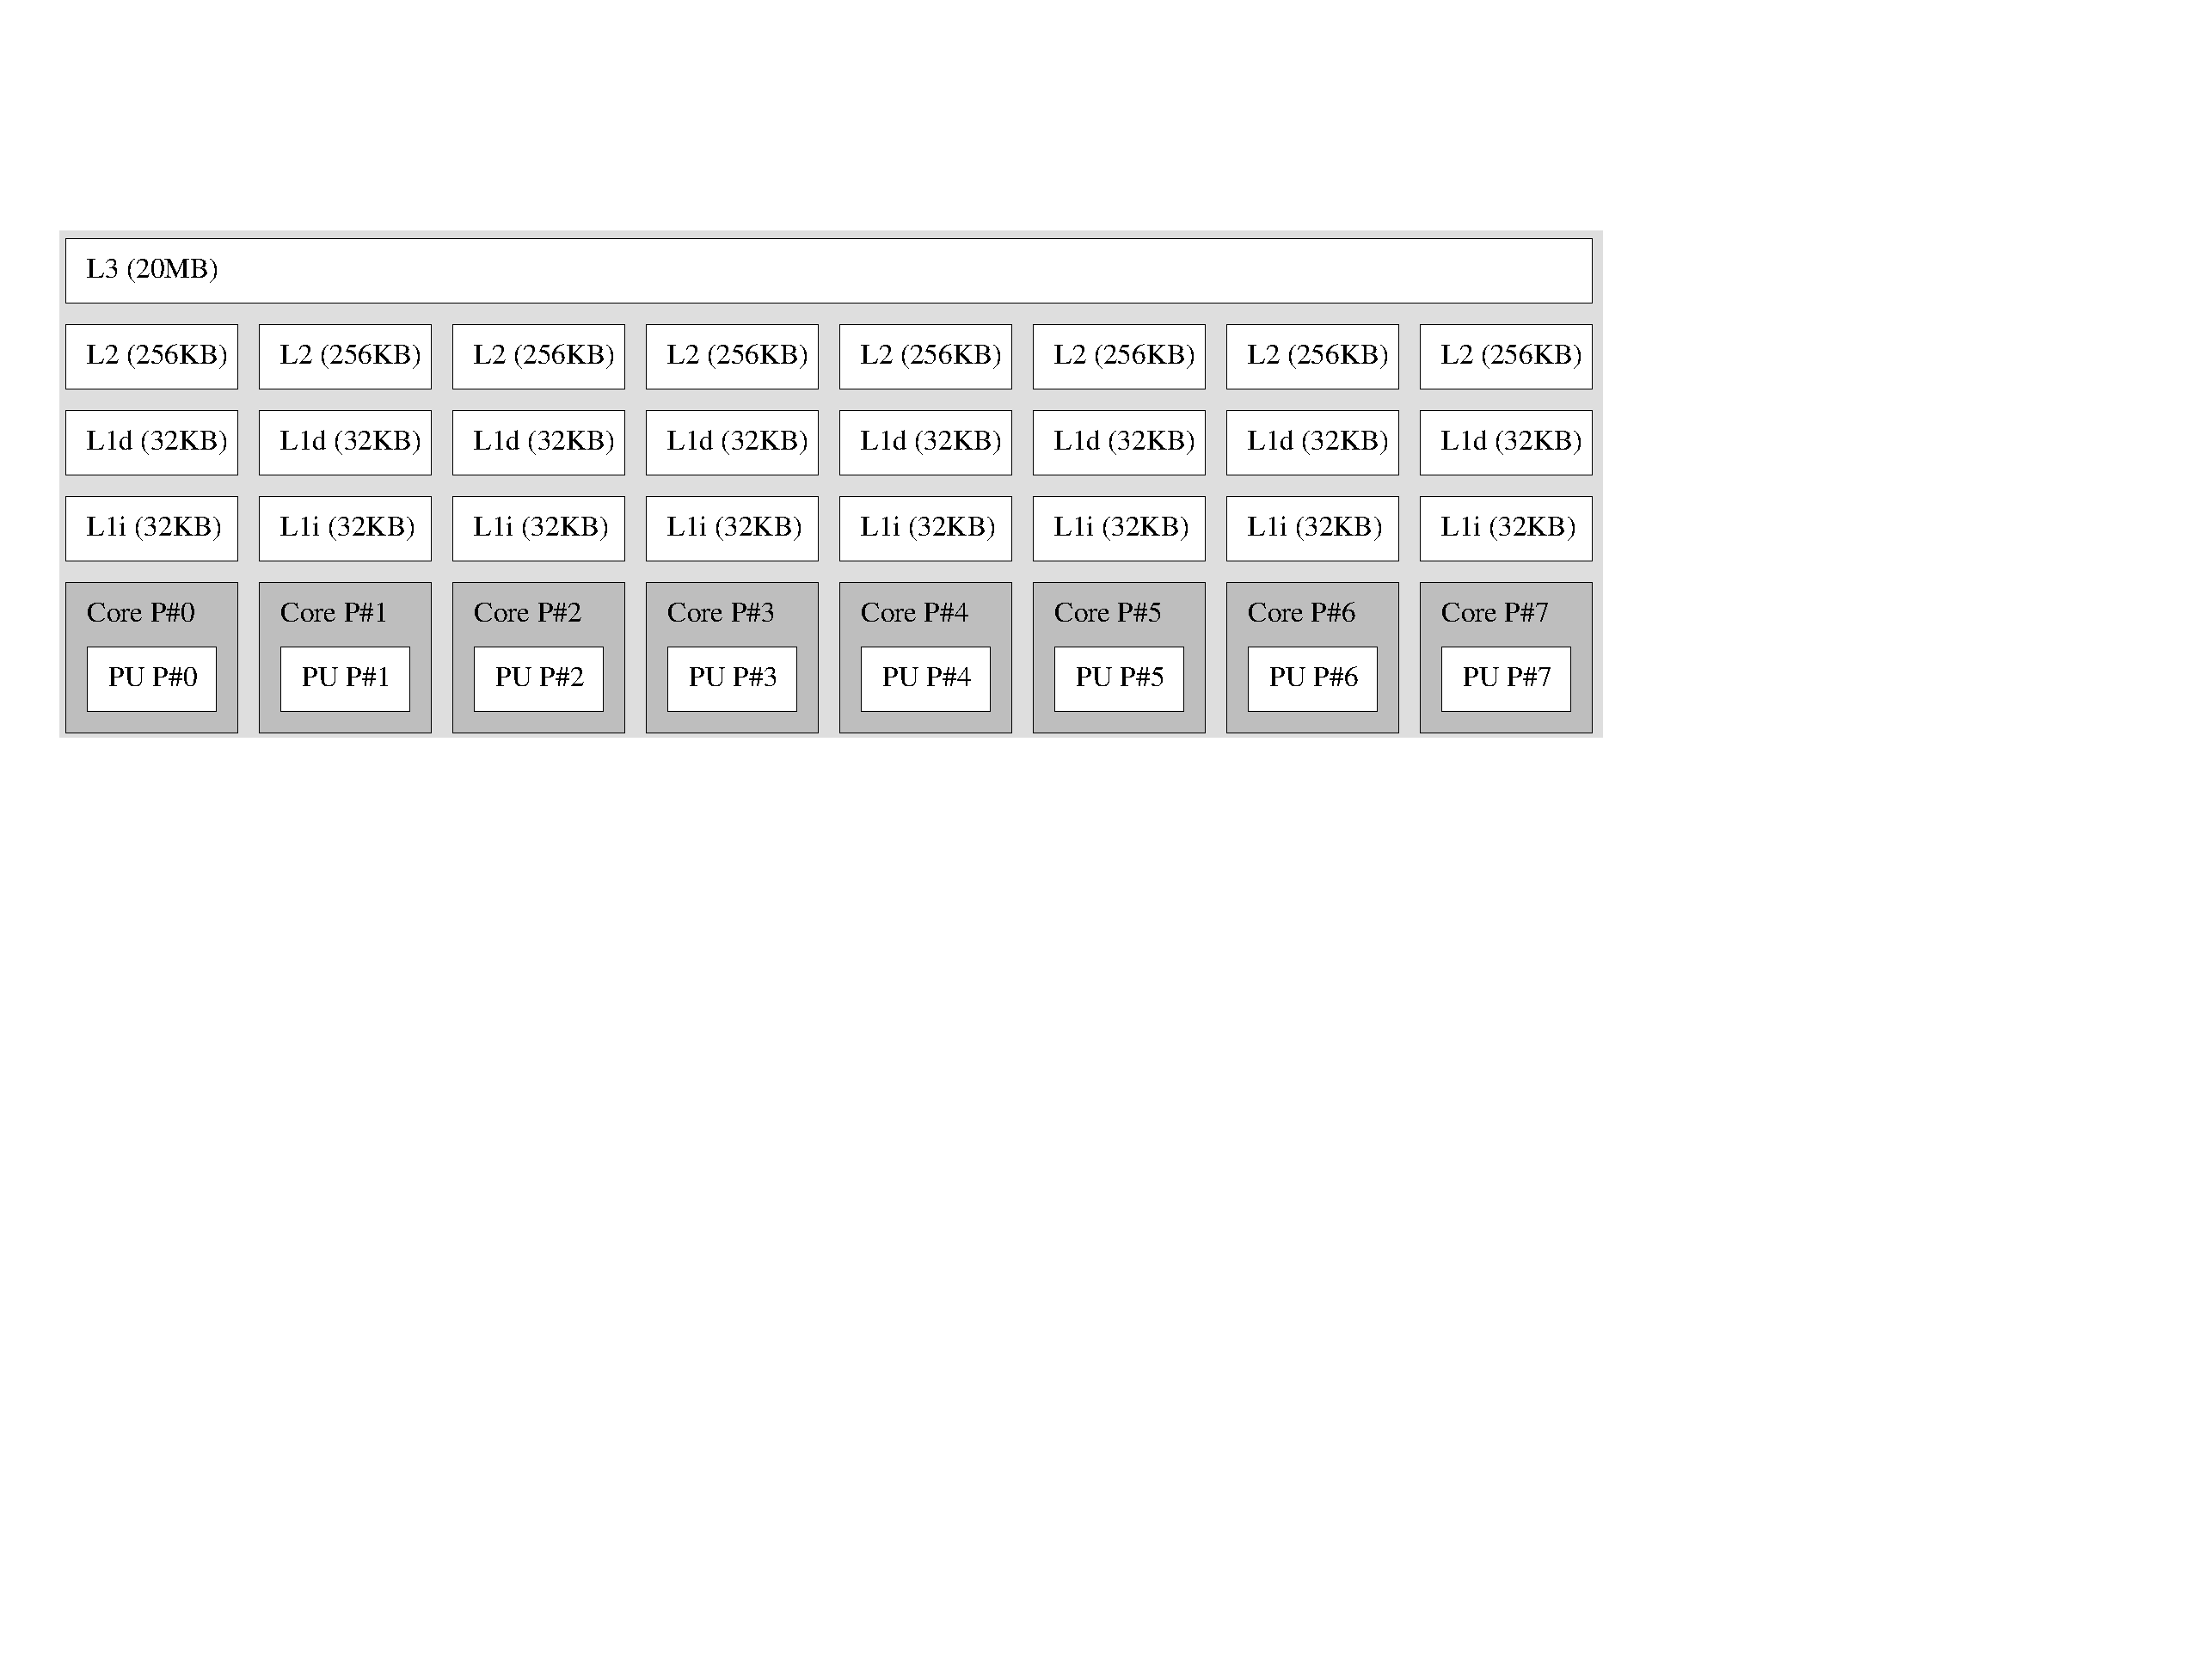
\includegraphics[width=12.5cm]{figures/cpu}}
%	\end{picture}
%}
%
%\frame{\frametitle{How Stampede nodes Looks Like?}
%	\begin{picture}(0,0)(0,0)
%		\put(-20,-210){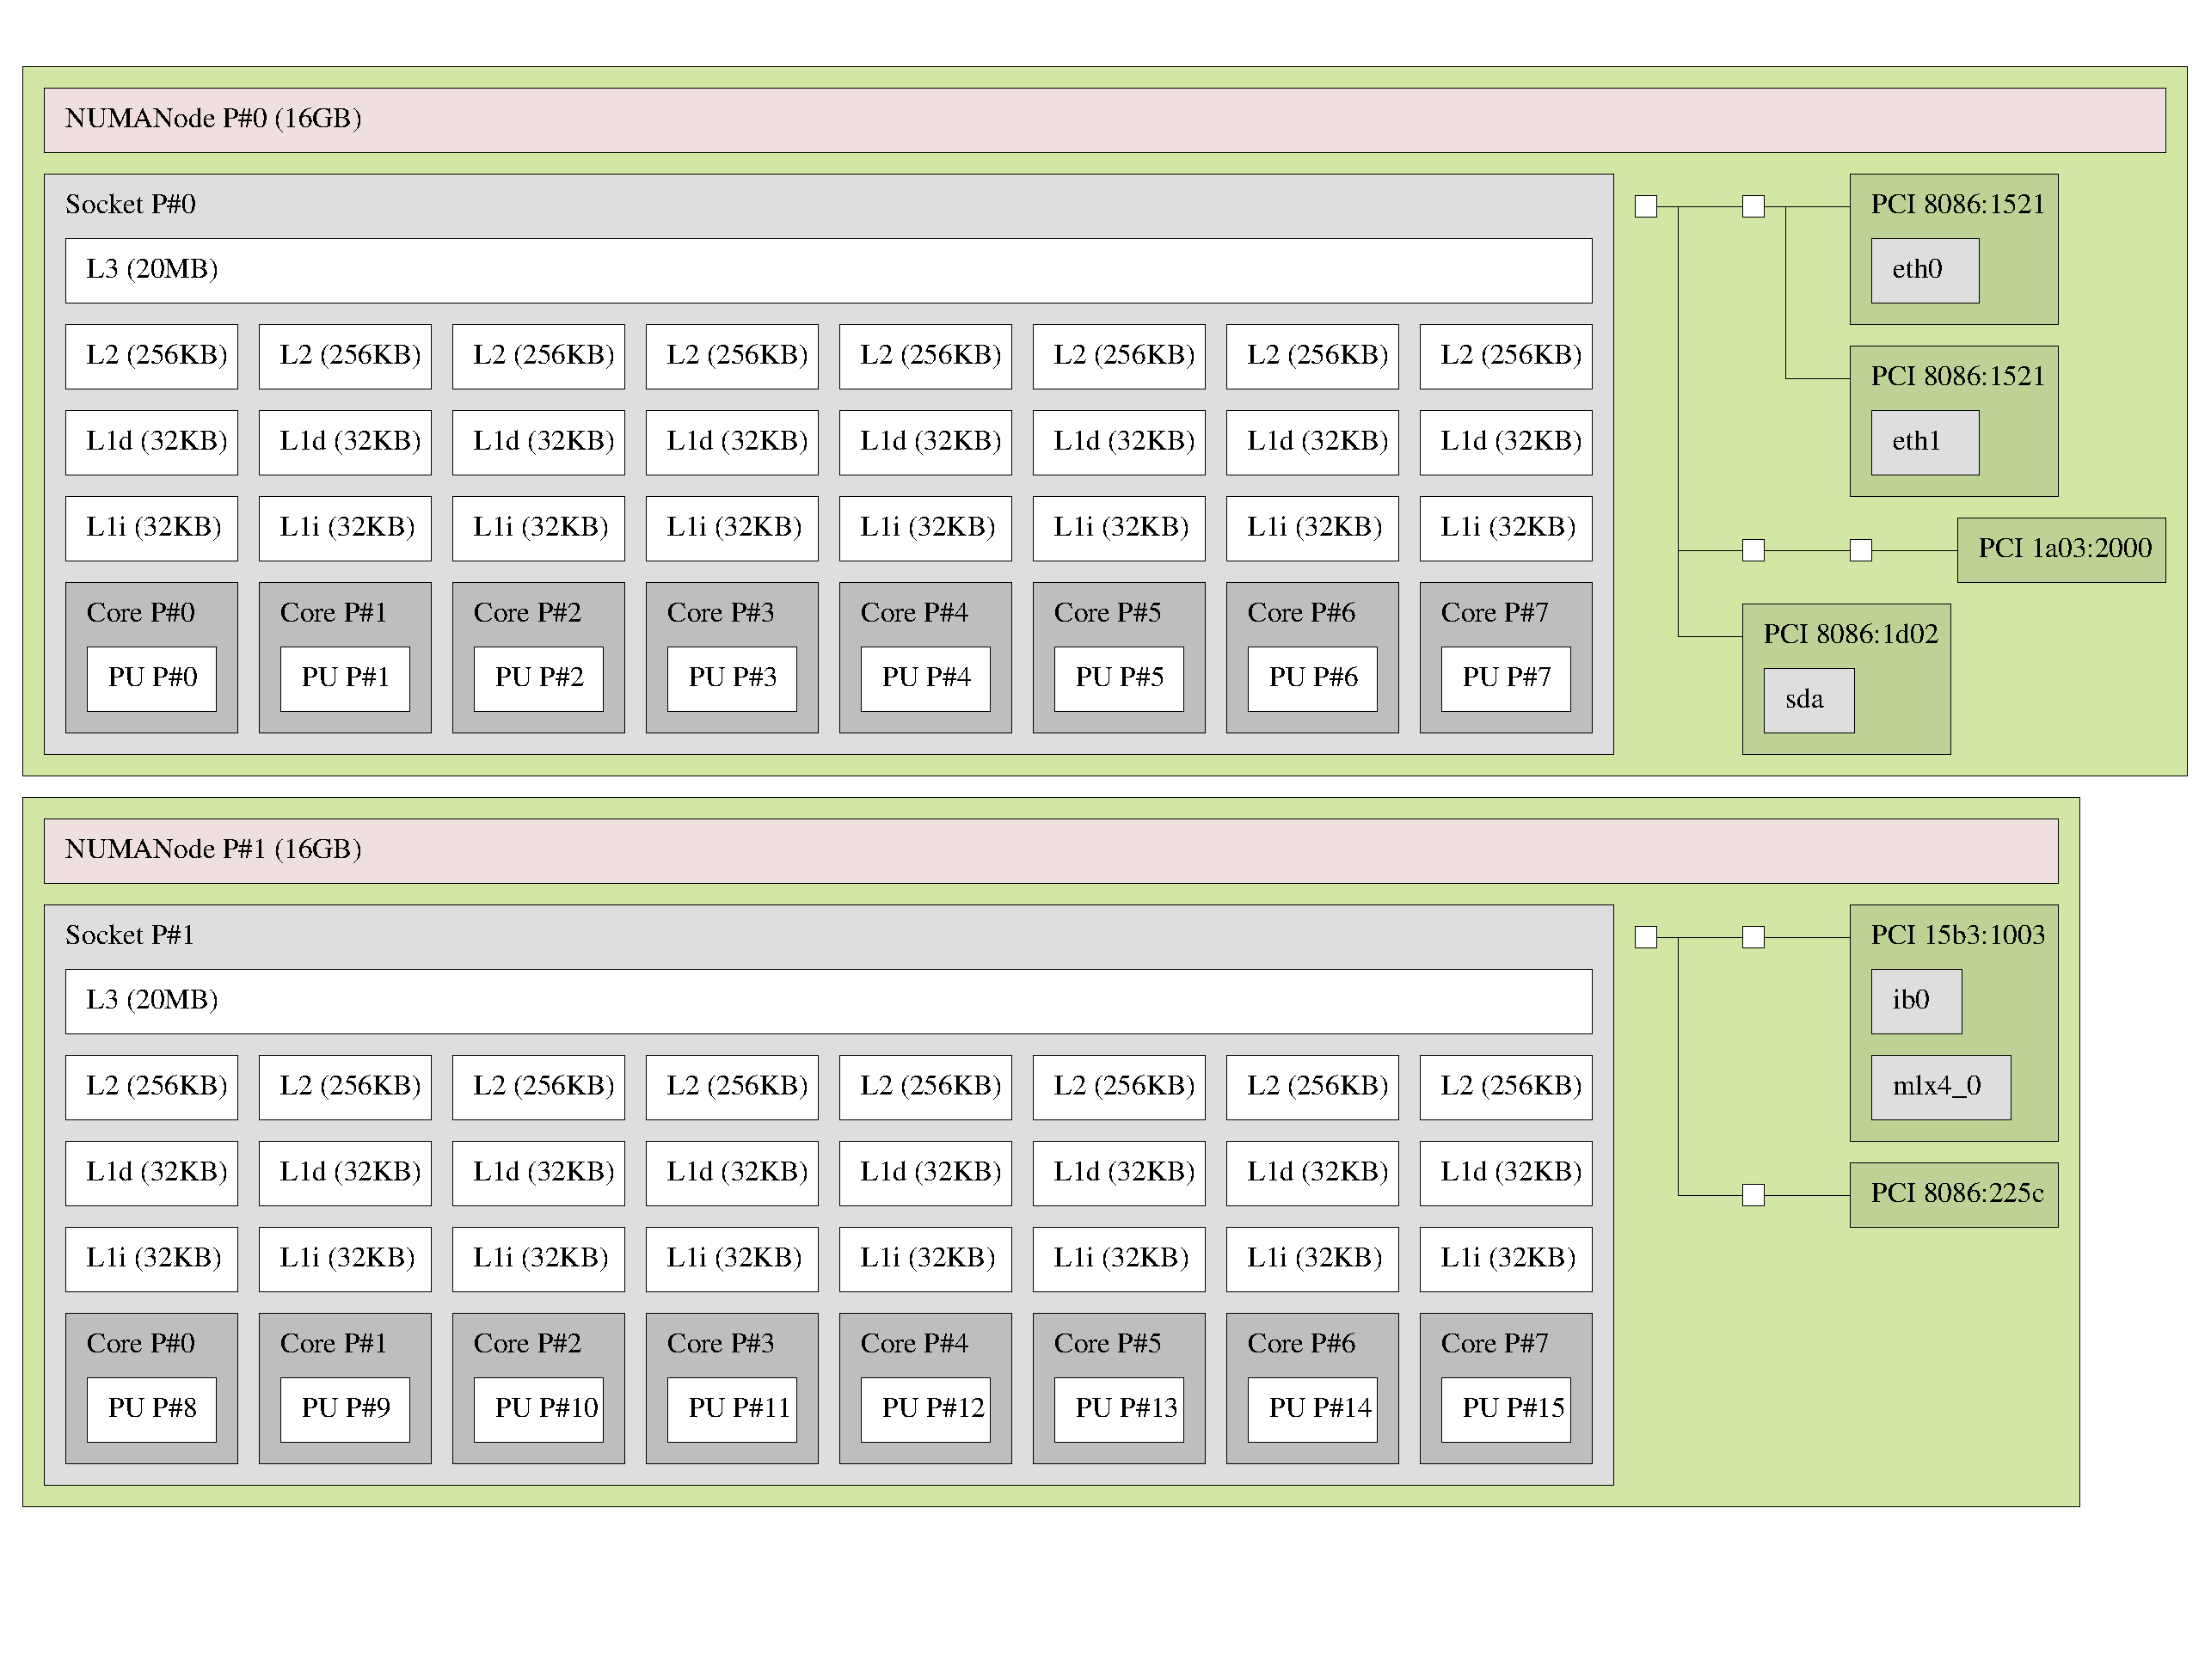
\includegraphics[width=12.2cm]{figures/node}}
%	\end{picture}
%}

%\subsection{Demo: PerfExpert}
%
%\frame{\frametitle{Short Demo}
%	\vspace{2.5cm}
%	\begin{center}
%		\textit{\textbf{\Huge{Short demo}}}
%	\end{center}
%}

%------------------------------------------------------------
\section{PerfExpert Modular Architecture}
\subsection{How PerfExpert does that?}

\frame{\frametitle{How PerfExpert does that: The Big Picture}
	\begin{picture}(0,0)(0,0)
		\put(-28,-160){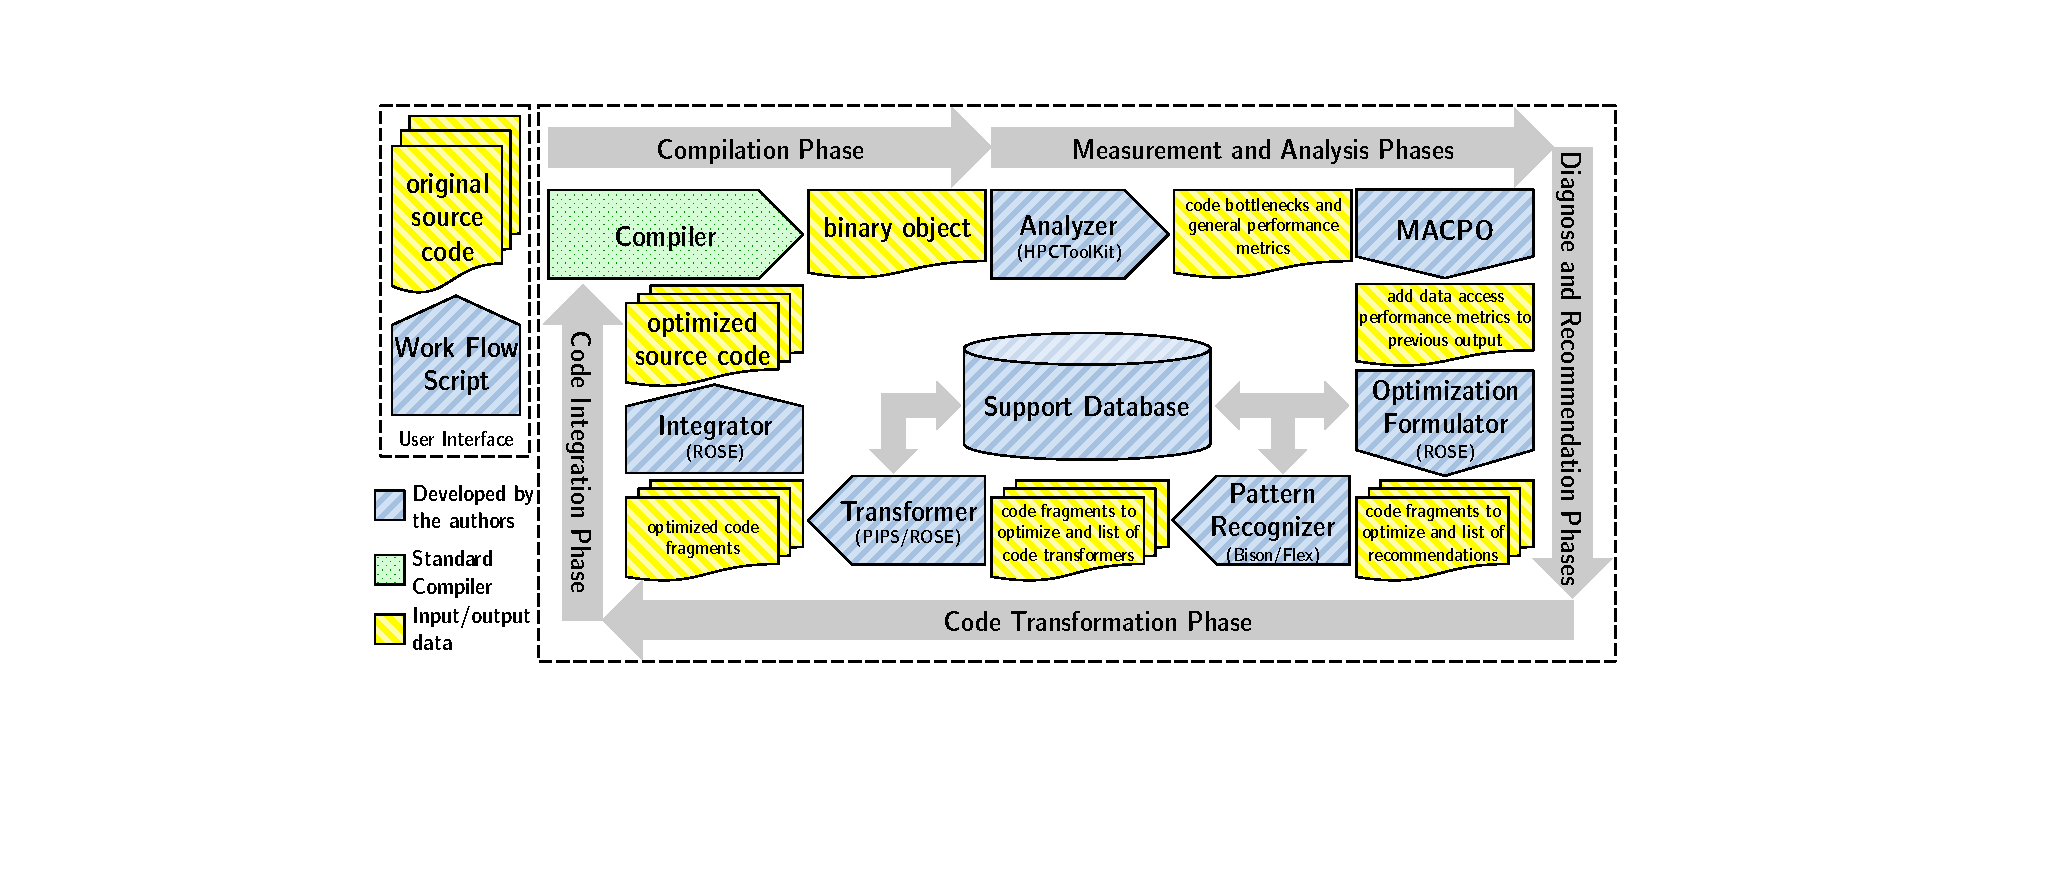
\includegraphics[width=12.8cm]{figures/pe_after}}
	\end{picture}
}

\frame{\frametitle{How PerfExpert does that: Work Flow Script}
	\begin{picture}(0,0)(0,0)
		\put(-28,-160){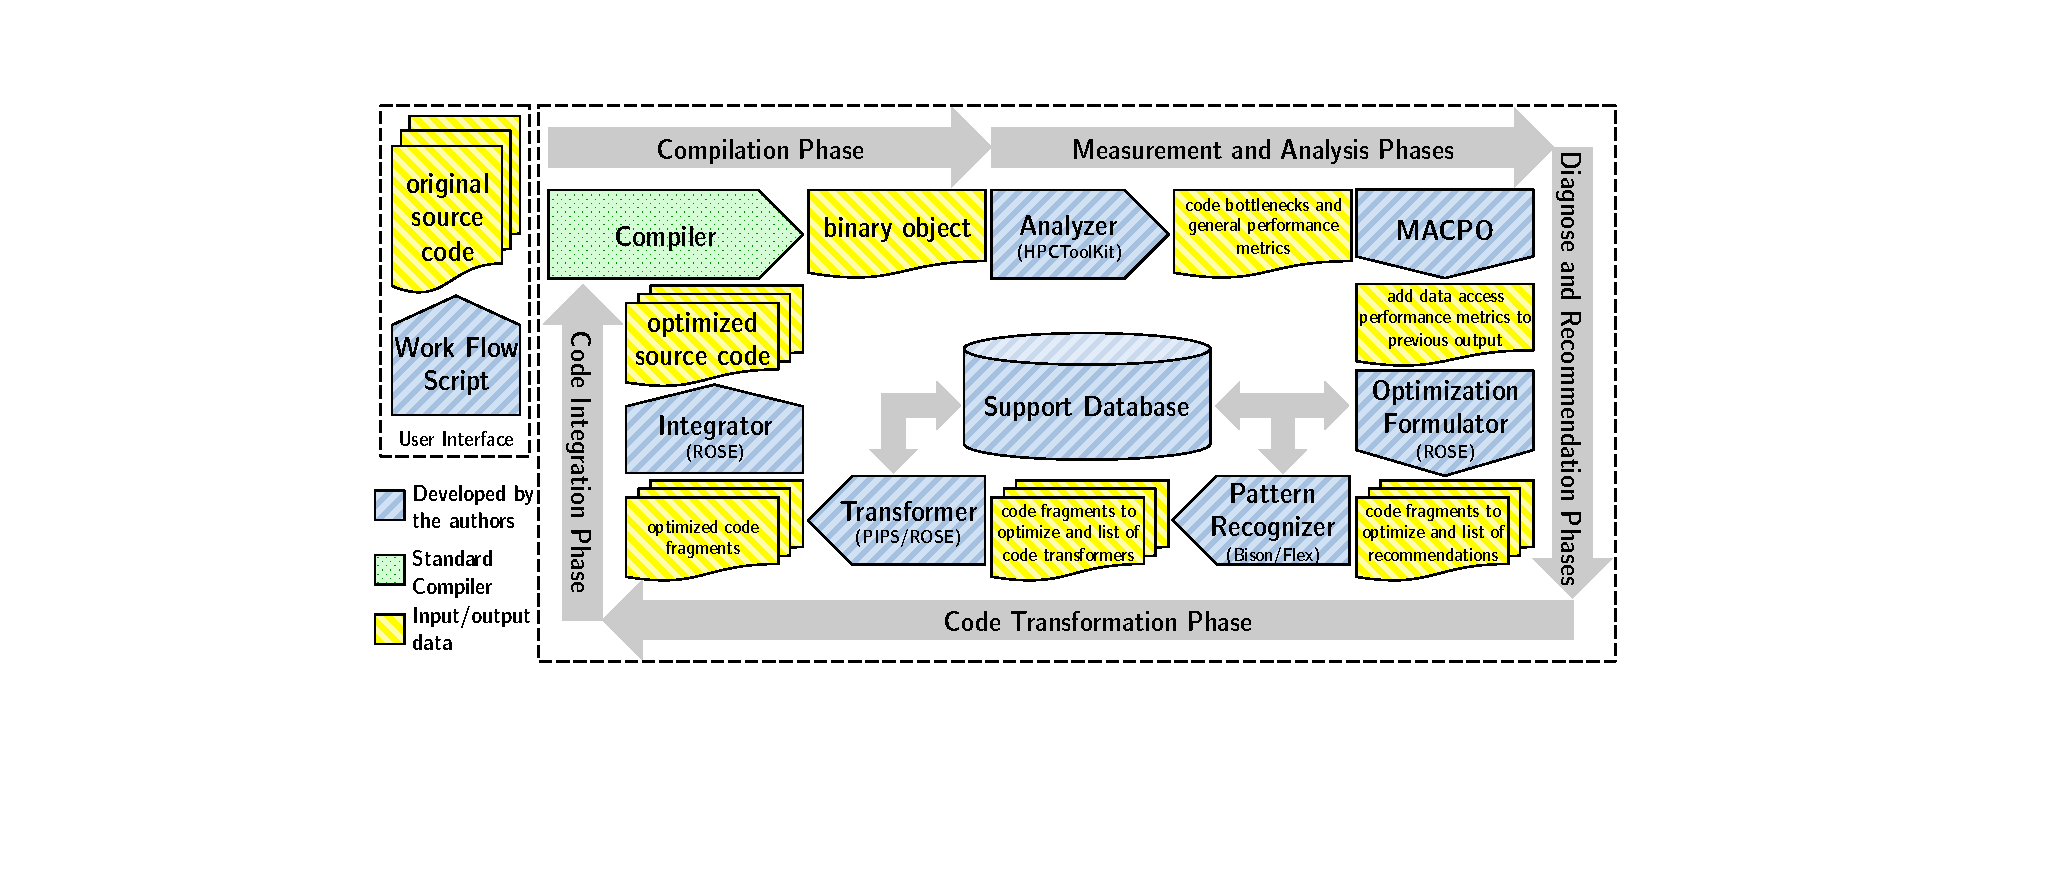
\includegraphics[width=12.8cm]{figures/pe_after}}
	\end{picture} %\pause
	\begin{columns}[c]
		\begin{column}{0.09\textwidth}
		\end{column}
		\begin{column}{0.43\textwidth}
			\vspace{1.5cm}
			\begin{block}{}
				\begin{itemize}
					\item This is a shell script \\[2mm] %\pause
					\item Accepts parameters \\[2mm] %\pause
					\item Invokes all tools (including the compiler) \\[2mm] %\pause
					\item Backward compatible \\[2mm]
				\end{itemize}
			\end{block}
		\end{column}
		\begin{column}{0.48\textwidth}
		\end{column}
	\end{columns}
}

\frame{\frametitle{How PerfExpert does that: Analyzer}
	\begin{picture}(0,0)(0,0)
		\put(-28,-160){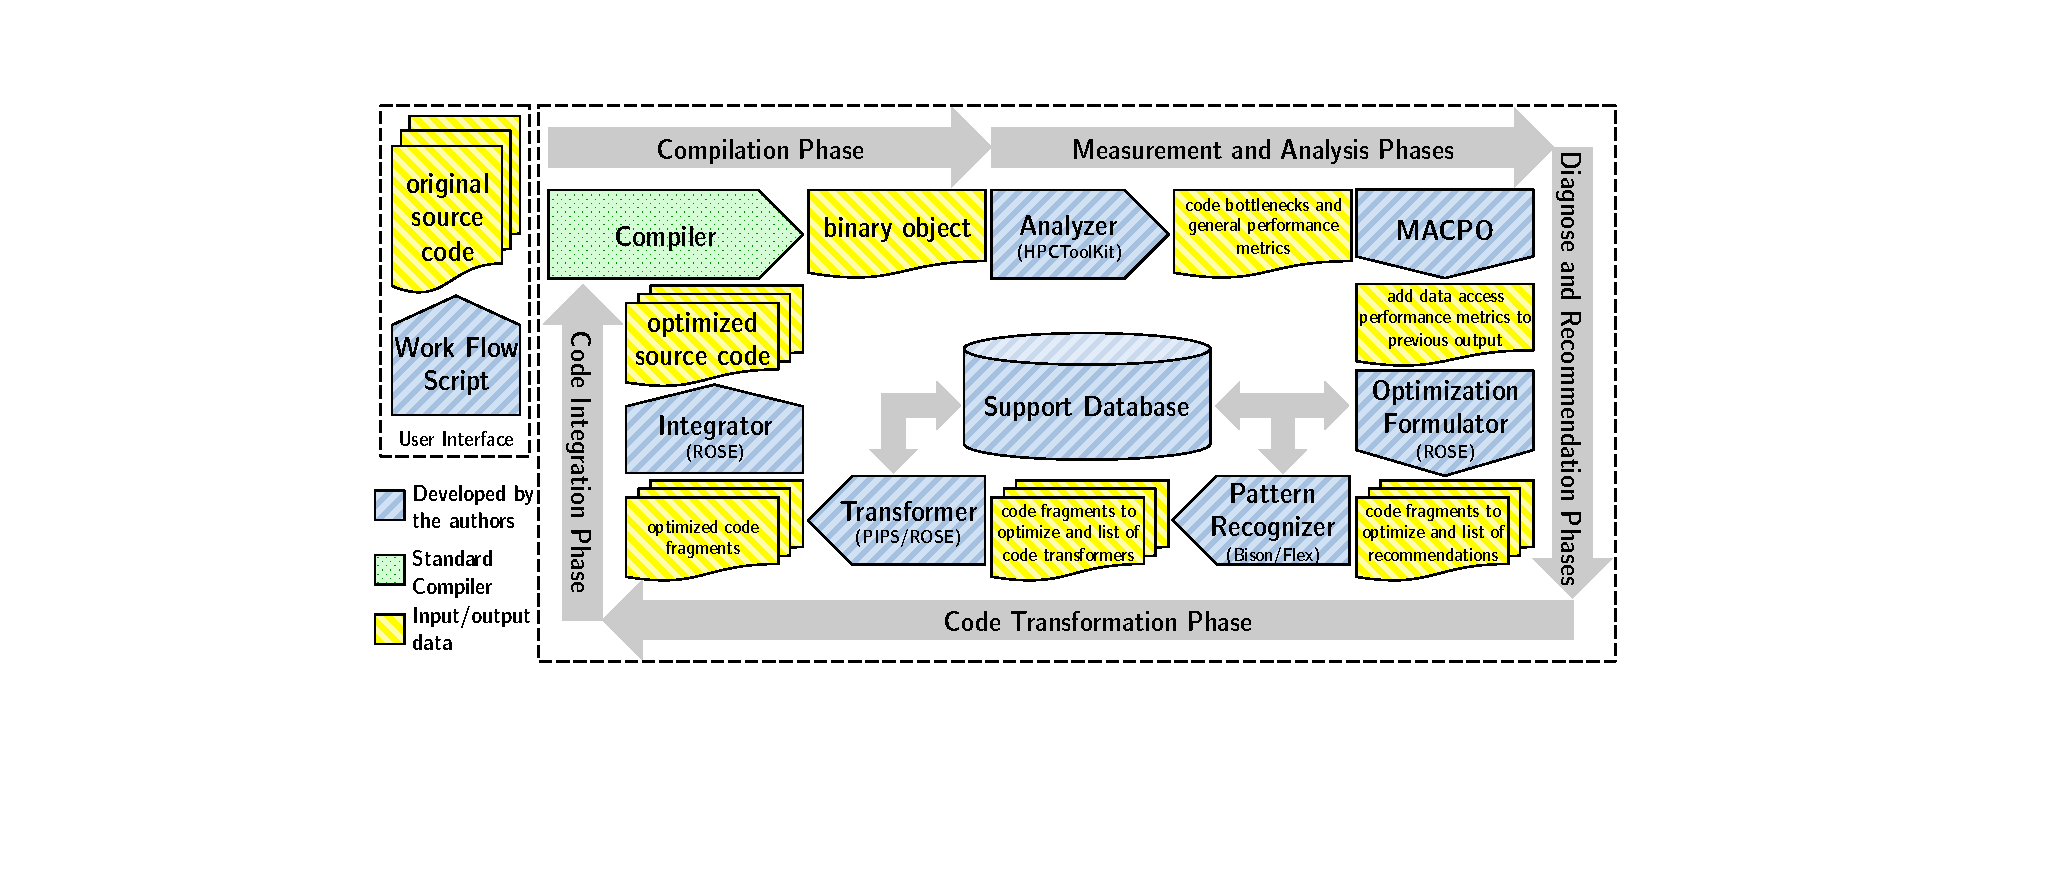
\includegraphics[width=12.8cm]{figures/pe_after}}
	\end{picture} %\pause
	\begin{columns}[c]
		\begin{column}{0.35\textwidth}
		\end{column}
		\begin{column}{0.46\textwidth}
			\vspace{1.5cm}
			\begin{block}{}
				\begin{itemize}
					\item This is the old PerfExpert, minus ``recommender'' \\[2mm] %\pause
					\item Based on HPCToolKit \\[2mm]
				\end{itemize}
			\end{block}
		\end{column}
		\begin{column}{0.19\textwidth}
		\end{column}
	\end{columns}
}

\frame{\frametitle{How PerfExpert does that: MACPO}
	\begin{picture}(0,0)(0,0)
		\put(-28,-160){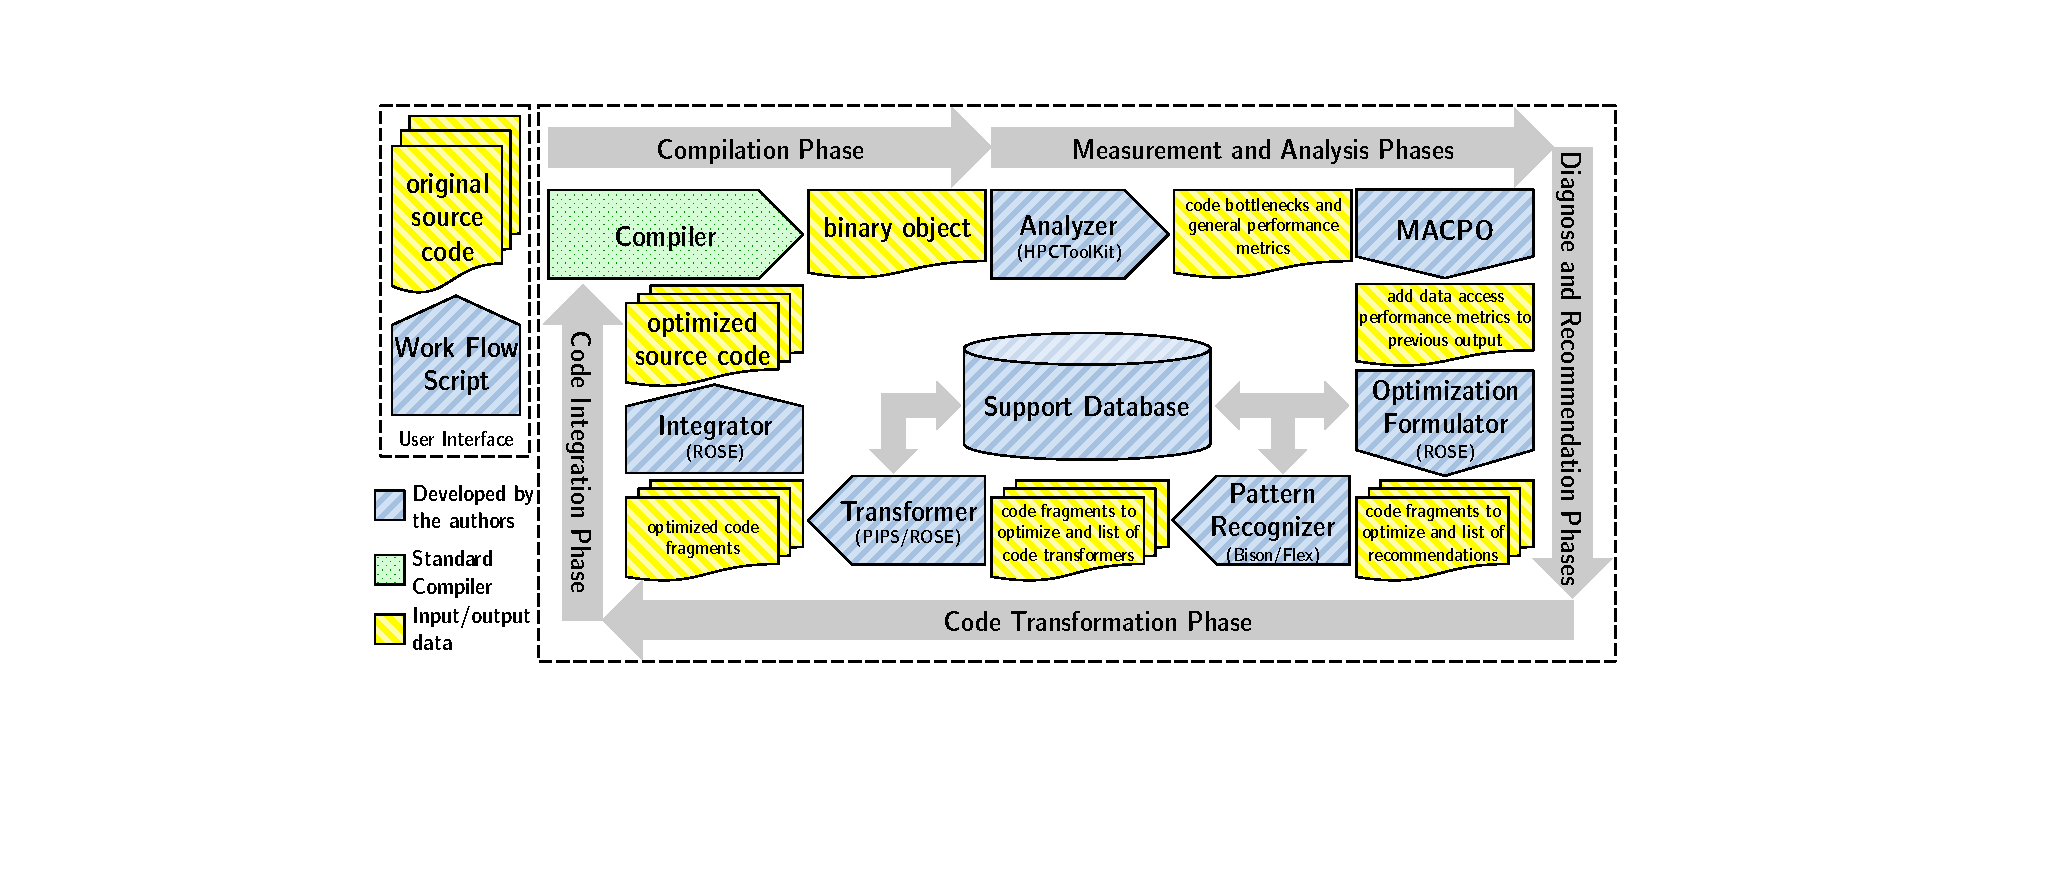
\includegraphics[width=12.8cm]{figures/pe_after}}
	\end{picture} %\pause
	\begin{columns}[c]
		\begin{column}{0.35\textwidth}
		\end{column}
		\begin{column}{0.46\textwidth}
			\vspace{1.5cm}
			\begin{block}{}
				\begin{itemize}
					\item Enhances the set of metrics with data access performance metrics \\[2mm] %\pause
					\item Based on ROSE \\[2mm]
				\end{itemize}
			\end{block}
		\end{column}
		\begin{column}{0.19\textwidth}
		\end{column}
	\end{columns}
}

\frame{\frametitle{How PerfExpert does that: Optimization Formulator}
	\begin{picture}(0,0)(0,0)
		\put(-28,-160){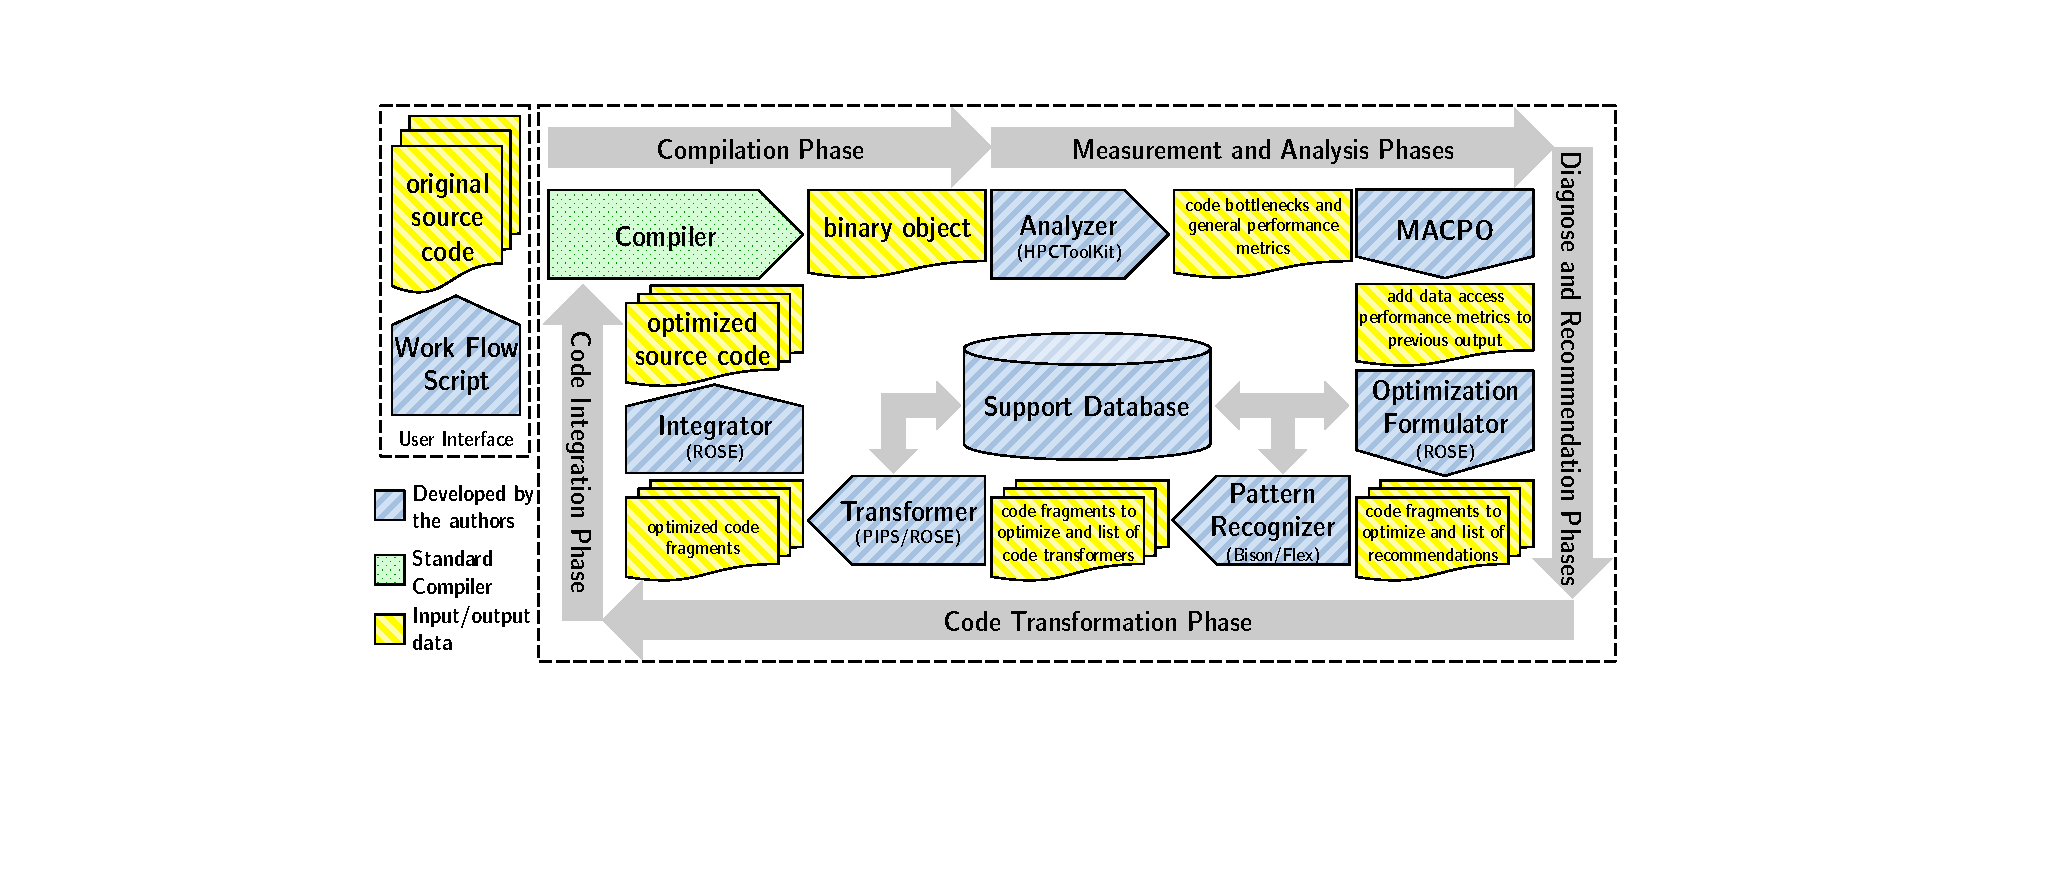
\includegraphics[width=12.8cm]{figures/pe_after}}
	\end{picture} %\pause
	\begin{columns}[c]
		\begin{column}{0.86\textwidth}
			\begin{block}{}
				\begin{itemize}
					\item Loads performance metrics on the Support Database \\[2mm] %\pause
					\item Runs all \textit{``recommendation selection functions''} \\[2mm] %\pause
					\item Concatenates and ranks the list of recommendations \\[2mm] %\pause
					\item Extracts code fragments identified as bottlenecks \\[2mm] %\pause
					\item Based on ROSE \\[2mm] %\pause
					\item \textbf{Extendable:} accepts user-defined performance metrics \\[2mm] %\pause
					\item \textbf{Extendable:} it is possible to write new \textit{``recommendation selection functions''} (SQL query) \\[2mm]
				\end{itemize}
			\end{block}
		\end{column}
		\begin{column}{0.19\textwidth}
		\end{column}
	\end{columns}
}

\frame{\frametitle{How PerfExpert does that: Support Database}
	\begin{picture}(0,0)(0,0)
		\put(-28,-160){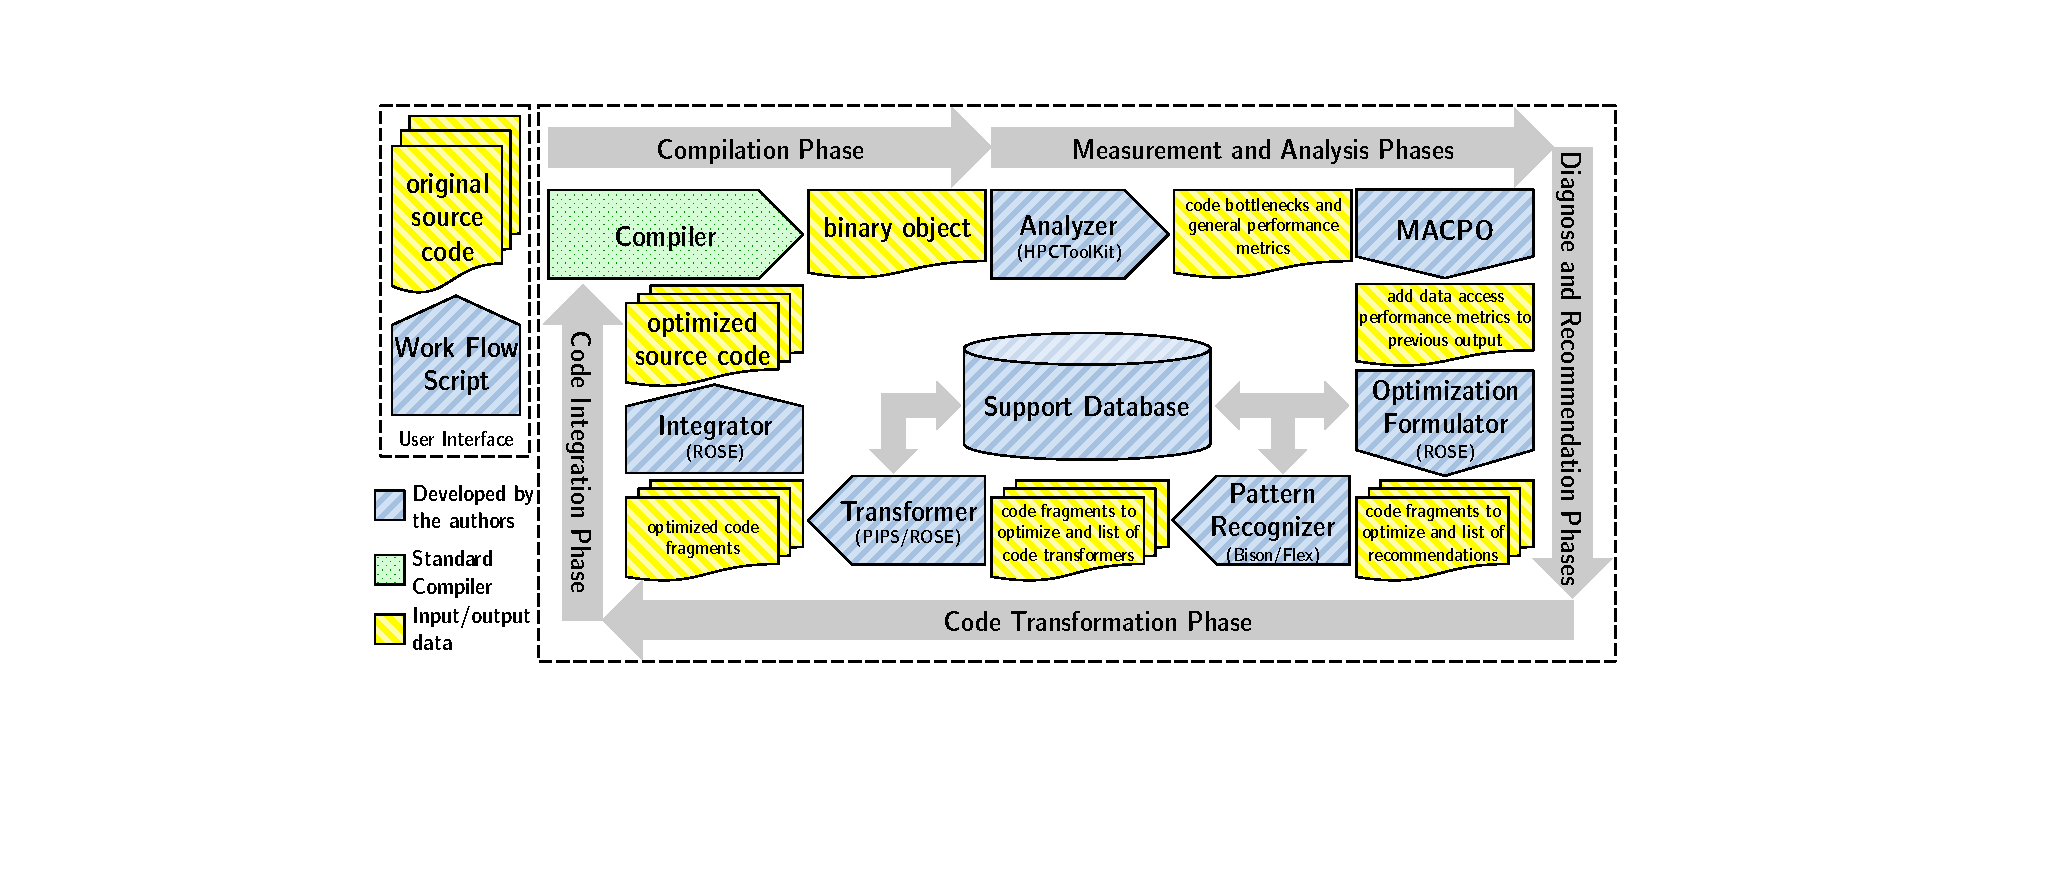
\includegraphics[width=12.8cm]{figures/pe_after}}
	\end{picture} %\pause
	\begin{columns}[c]
		\begin{column}{0.1\textwidth}
		\end{column}
		\begin{column}{0.96\textwidth}
			\vspace{-0.8cm}
			\begin{block}{}
				\begin{itemize}
					\item This is a SQLite database \\[2mm] %\pause
					\item Stores the list of \textit{``recommendation selection functions''}, \textit{``pattern recognizers''} and \textit{``code transformers''} \\[2mm] %\pause
					\item Engine to run the \textit{``recommendation selection functions''}
				\end{itemize}
			\end{block}
		\end{column}
	\end{columns}
}

\frame{\frametitle{How PerfExpert does that: Pattern Recognizer}
	\begin{picture}(0,0)(0,0)
		\put(-28,-160){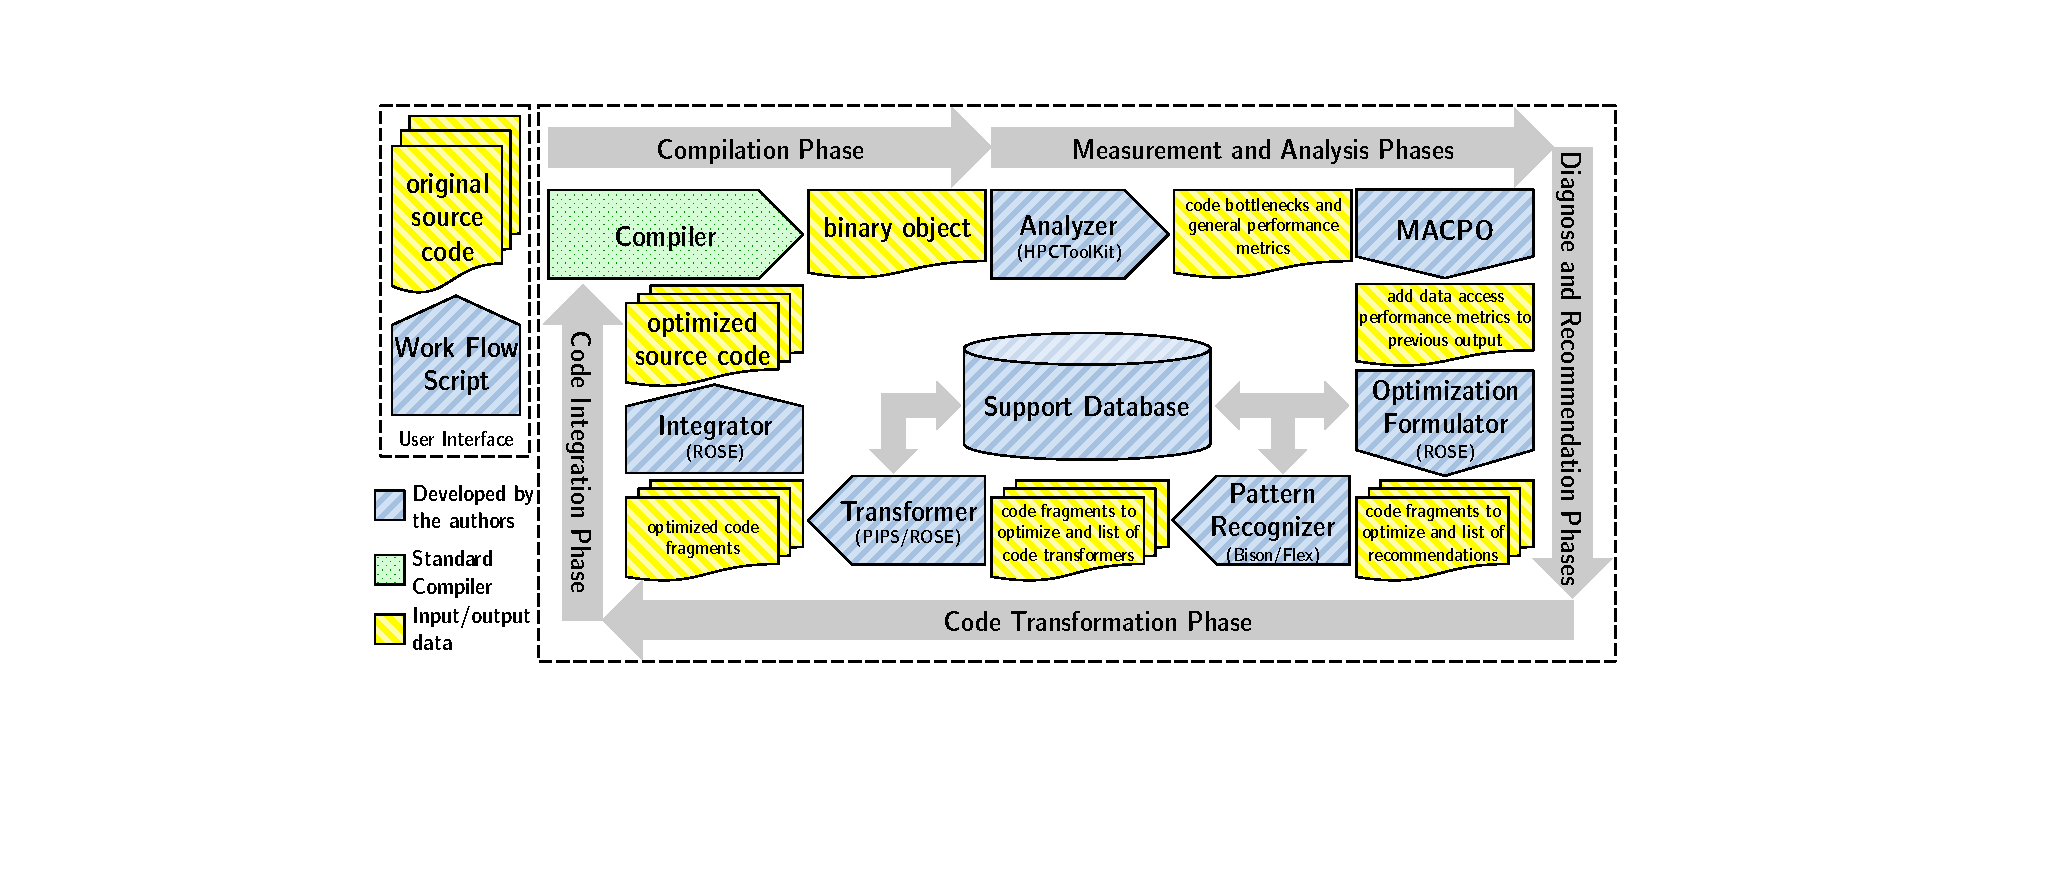
\includegraphics[width=12.8cm]{figures/pe_after}}
	\end{picture} %\pause
	\begin{columns}[c]
		\begin{column}{0.05\textwidth}
		\end{column}
		\begin{column}{1.05\textwidth}
			\vspace{-1.2cm}
			\begin{block}{}
				\begin{itemize}
					\item Acts as a ``filter'' trying to find (match) the right code transformer for a source code fragment (identified as bottleneck) \\[2mm] %\pause
					\item Language sensitive \\[2mm] %\pause
					\item Based on Bison and Flex \\[2mm] %\pause
					\item One recommendation may have multiple pattern recognizers \\[2mm] %\pause
					\item \textbf{Extendable:} it is possible to write new grammars to recognize/ match/filter code fragments (to work with new ``transformers'') \\[2mm]
				\end{itemize}
			\end{block}
		\end{column}
	\end{columns}
}

\frame{\frametitle{How PerfExpert does that: Transformer}
	\begin{picture}(0,0)(0,0)
		\put(-28,-160){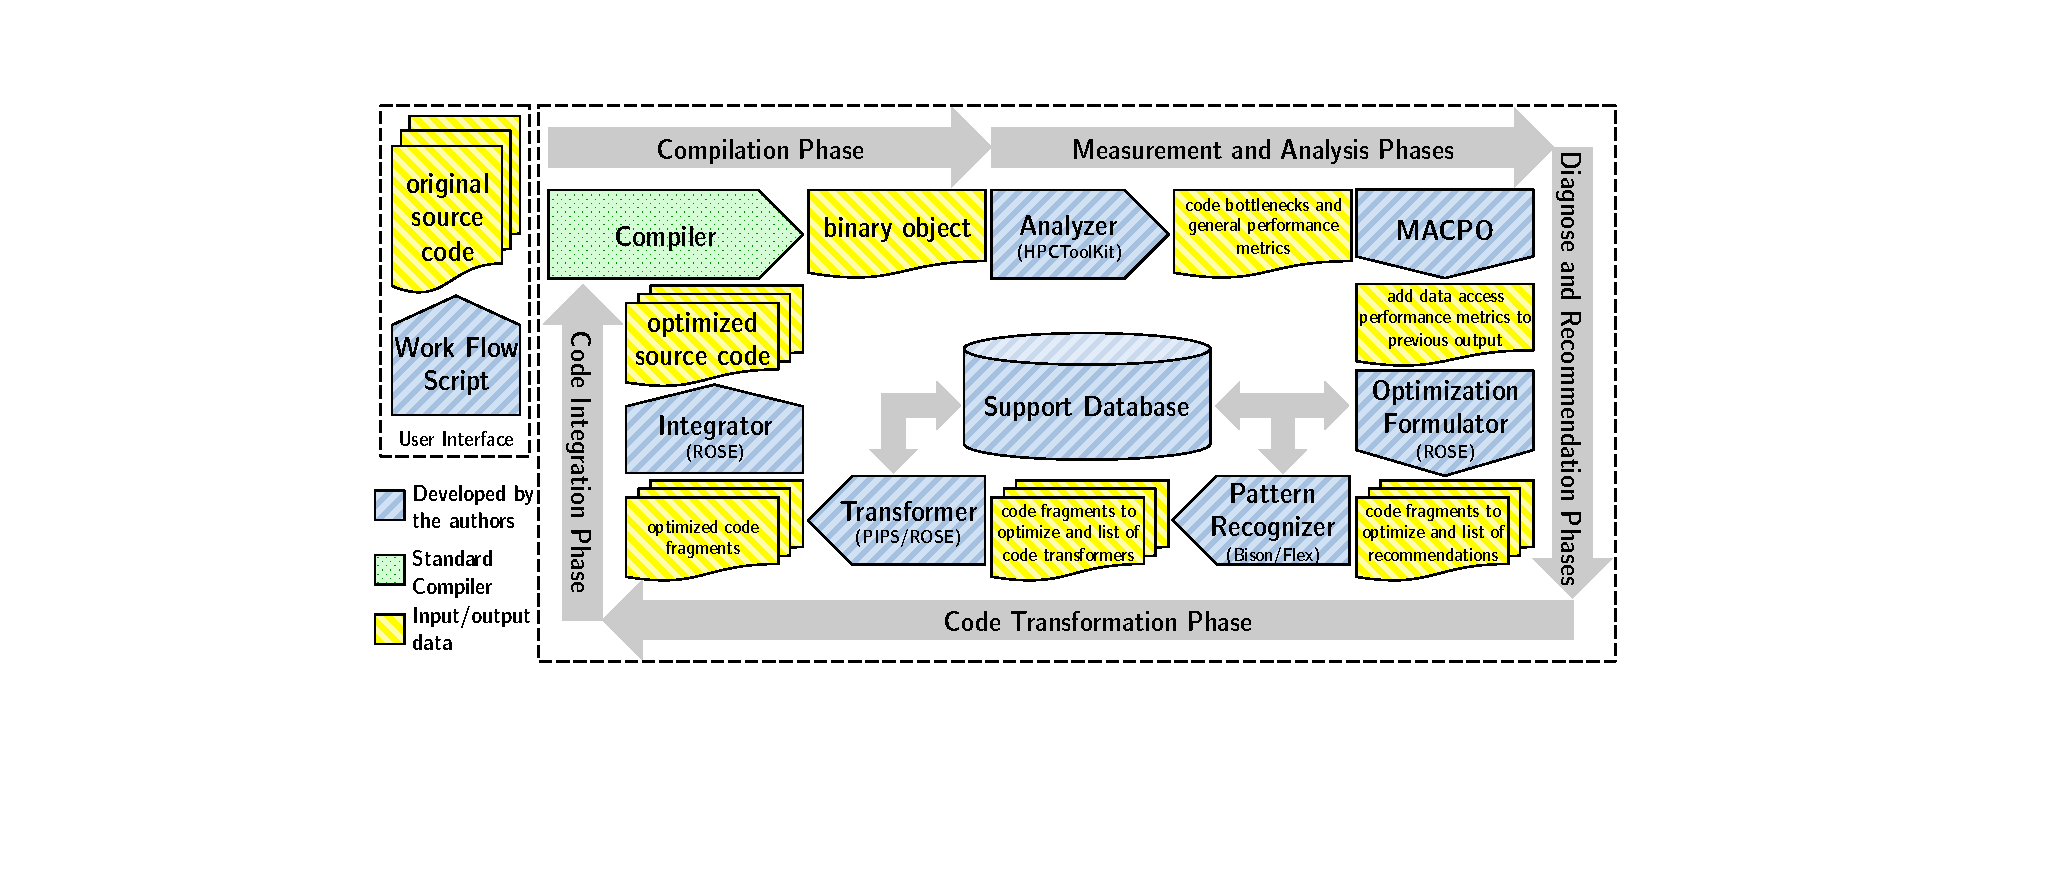
\includegraphics[width=12.8cm]{figures/pe_after}}
	\end{picture} %\pause
	\vspace{-1.1cm}
	\begin{block}{}
		\begin{itemize}
			\item Implements the recommendation by applying source code transformation \\[2mm] %\pause
			\item May or may not be language sensitive \\[2mm] %\pause
			\item Based on ROSE, PIPS or anything you want \\[2mm] %\pause
			\item One code pattern may lead to multiple code transformers \\[2mm] %\pause
			\item \textbf{Extendable:} it is possible to write code transformers using any language you want \\[2mm]
		\end{itemize}
	\end{block}
}

\frame{\frametitle{How PerfExpert does that: Integrator}
	\begin{picture}(0,0)(0,0)
		\put(-28,-160){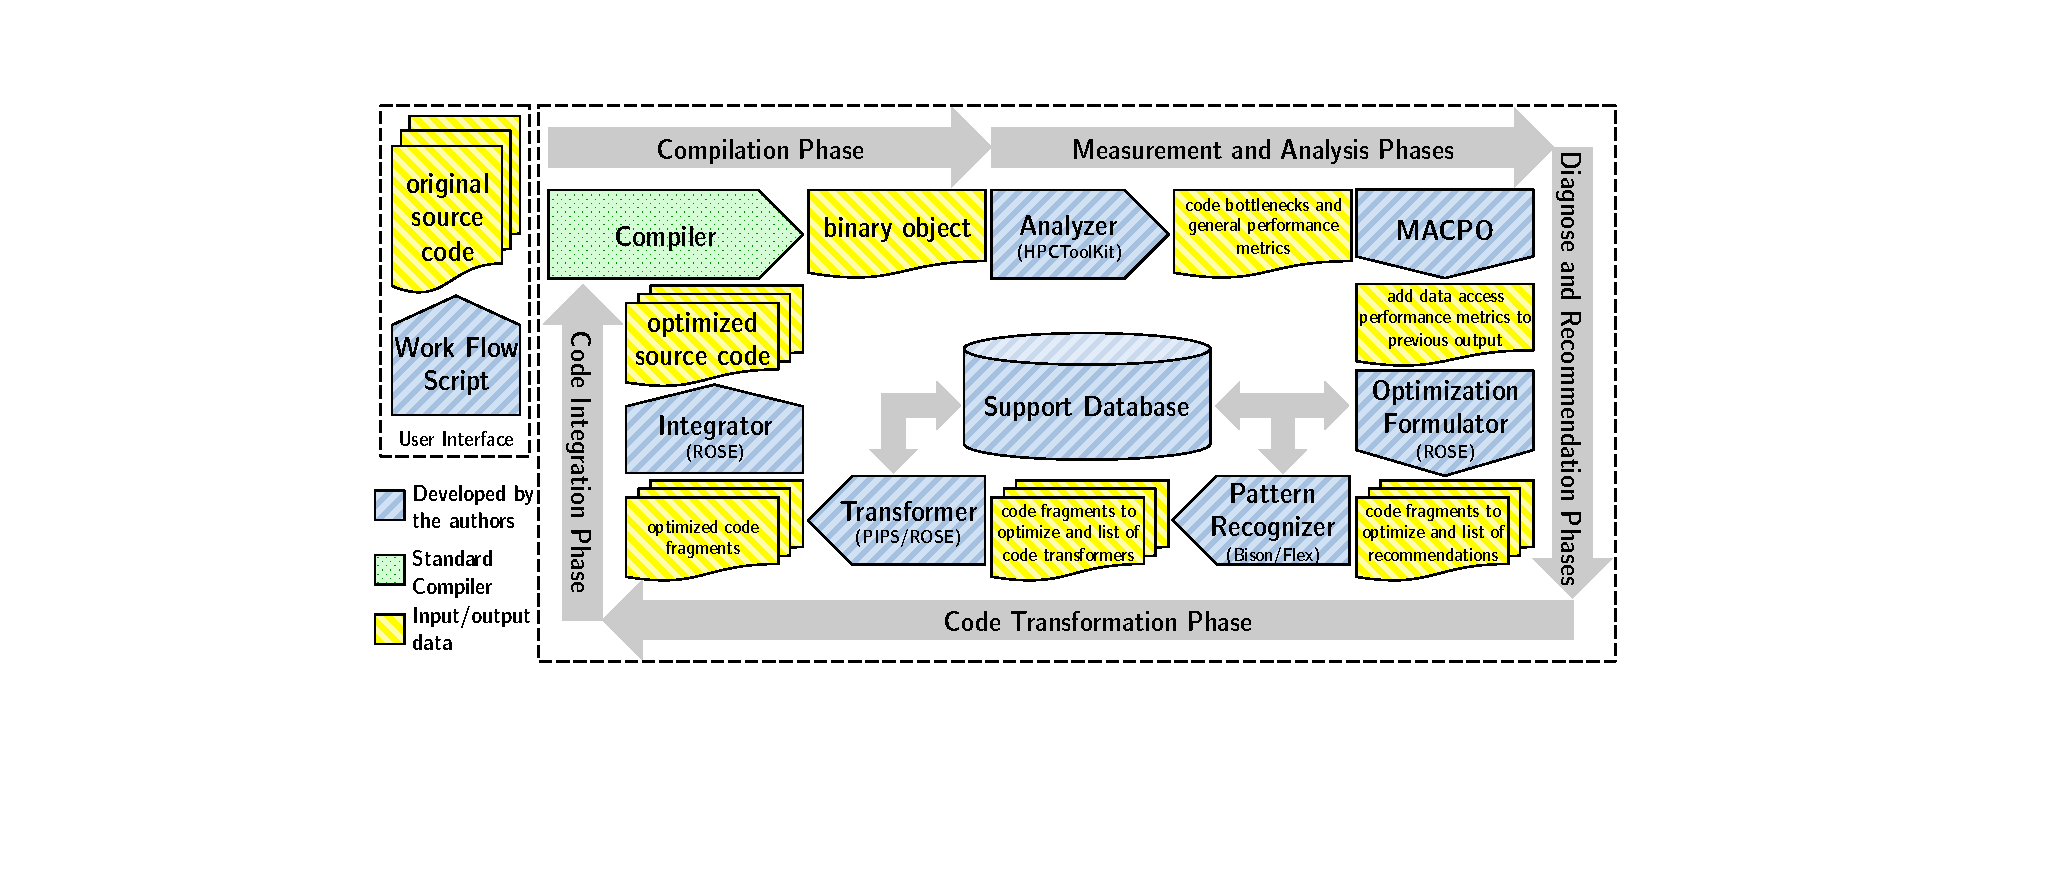
\includegraphics[width=12.8cm]{figures/pe_after}}
	\end{picture} %\pause
	\begin{columns}[c]
		\begin{column}{0.35\textwidth}
		\end{column}
		\begin{column}{0.46\textwidth}
			\vspace{1.5cm}
			\begin{block}{}
				\begin{itemize}
					\item Generates a new source code by integrating to the transformed code fragments \\[2mm] %\pause
					\item Based on ROSE \\[2mm]
				\end{itemize}
			\end{block}
		\end{column}
		\begin{column}{0.19\textwidth}
		\end{column}
	\end{columns}
}

\frame{\frametitle{How PerfExpert does that: Key Points} %\pause
	\begin{block}{Why is this performance optimization ``architecture'' strong?} %\pause
		\begin{itemize}
			\item Each piece of the tool chain can be updated/upgraded individually \\[2mm] %\pause
			\item It is flexible: you can add new metrics as well as plug new tools to measure application performance \\[2mm] %\pause
			\item \textbf{It is extendable}: new recommendations, transformations and strategies to select recommendations \\[2mm] %\pause
			\item Multi-language, \textbf{multi-architecture}, open-source and built on top of well-established tools (HPCToolKit, ROSE, PIPS, etc.) \\[2mm] %\pause
			\item Easy to use and lightweight!
		\end{itemize}
	\end{block}
}

%------------------------------------------------------------
%\section{Understanding and Extending PerfExpert}
%\subsection{Understanding and Extending PerfExpert}
%
%\frame{\frametitle{Understanding PerfExpert} %\pause
%	\begin{block}{} %\pause
%		\begin{itemize}
%			\item Performance metrics \\[2mm] %\pause
%			\item Optimization recommendations \\[2mm] %\pause
%			\item ``Recommendation selection functions'' \\[2mm] %\pause
%			\item Pattern recognizers \\[2mm] %\pause
%			\item Code transformers \\[2mm]
%		\end{itemize}
%	\end{block}
%}
%
%\frame{\frametitle{Optimization recommendations} %\pause
%	\begin{block}{Recommendations consists of...} %\pause
%%		\begin{itemize}
%%			\item  \\[2mm] %\pause
%%			\item  \\[2mm] %\pause
%%			\item 
%%		\end{itemize}
%	\end{block}
%}
%
%\frame{\frametitle{Recommendation Selection Functions} %\pause
%	\begin{block}{Picking up recommendations} %\pause
%%		\begin{itemize}
%%			\item The basic idea: \textbf{\texttt{SELECT id FROM recommendation WHERE metric.x > 'whatever' ORDER BY score DESC;}} \\[2mm] %\pause
%%			\item Every selection function will be executed to find the best recommendations \\[2mm] %\pause
%%			\item 
%%		\end{itemize}
%	\end{block}
%}
%
%\frame{\frametitle{Pattern Recognizers} %\pause
%	\begin{block}{Checking the feasibility of transformation} %\pause
%%		\begin{itemize}
%%			\item  \\[2mm] %\pause
%%			\item  \\[2mm] %\pause
%%			\item 
%%		\end{itemize}
%	\end{block}
%}
%
%\frame{\frametitle{Code Transformers} %\pause
%	\begin{block}{Applying recommendation to the source code} %\pause
%%		\begin{itemize}
%%			\item  \\[2mm] %\pause
%%			\item  \\[2mm] %\pause
%%			\item 
%%		\end{itemize}
%	\end{block}
%}

%------------------------------------------------------------
\section{Conclusions}
\subsection{Conclusions}
\frame{\frametitle{Conclusions} %\pause
	\begin{block}{}
		\begin{itemize}
			\item This is the first end-to-end open-source performance optimization tool (as far as we know)\\[2mm] %\pause
			\item It will become more and more powerful as new recommendations, transformations and features are added \\[2mm] %\pause
			\item Different from (most of) the available performance optimization tools, there is no ``big code'' (to increase in complexity until it become unusable or too hard to maintain) \\[2mm]
		\end{itemize}
	\end{block}
}

\frame{\frametitle{Next Steps} %\pause
	\begin{block}{Major Goals} %\pause
		\begin{itemize}
			\item Improve analysis based on the data access \textcolor{red}{(in progress)} \\[2mm] %\pause
			\item Increase the number of recommendations and possible code transformations \textcolor{red}{(continuously)} \\[2mm] %\pause
			\item New algorithms for recommendations selection \textcolor{red}{(in progress)} \\[2mm] %\pause
			\item Add support to MIC architecture \textcolor{red}{(in progress)} \\[2mm] %\pause
			\item Add support to MPI-related recommendations (medium term) \\[2mm] %\pause
			\item Add support to MPI-related code transformations (long term) \\[2mm] %\pause
		\end{itemize}
	\end{block}
}

\frame{\frametitle{Next Steps} %\pause
	\begin{block}{Minor Goals} %\pause
		\begin{itemize}
			\item Support ``Makefile''-based source code/compilation tree \textcolor{red}{(done!)} \\[2mm] %\pause
			\item Make the required packages installation process easier \textcolor{red}{(done!)} \\[2mm] %\pause
			\item Add a test suite based on established benchmark codes \textcolor{red}{(in progress)} \\[2mm] %\pause
			\item Easy-to-use interface to manipulate the support database \textcolor{red}{(medium term)} \\[2mm]
		\end{itemize}
	\end{block}
}

\frame[plain]{
	\vspace{2cm}
	\begin{center}
		\textbf{\Huge{Thank You\\ \ \\ fialho@utexas.edu}}
	\end{center}
	\vspace{1cm}
	\pgfuseimage{logo_TACC} \ \ \pgfuseimage{logo_UT}
}

%------------------------------------------------------------
\end{document}